\chapter{Diseño}

\section{SRD como afilador de flanco}
\label{sec:srd_sharpener}

En la sección \textcolor{red}{AGREGAR REF\ref{TODO}} fue explicado como un diodo
\textit{SRD} funciona como afilador de flanco.

En la figura \ref{fig:srd_sharpener} puede observarse un circuito que demuestra
el funcionamiento.

\begin{figure}
  \centering
    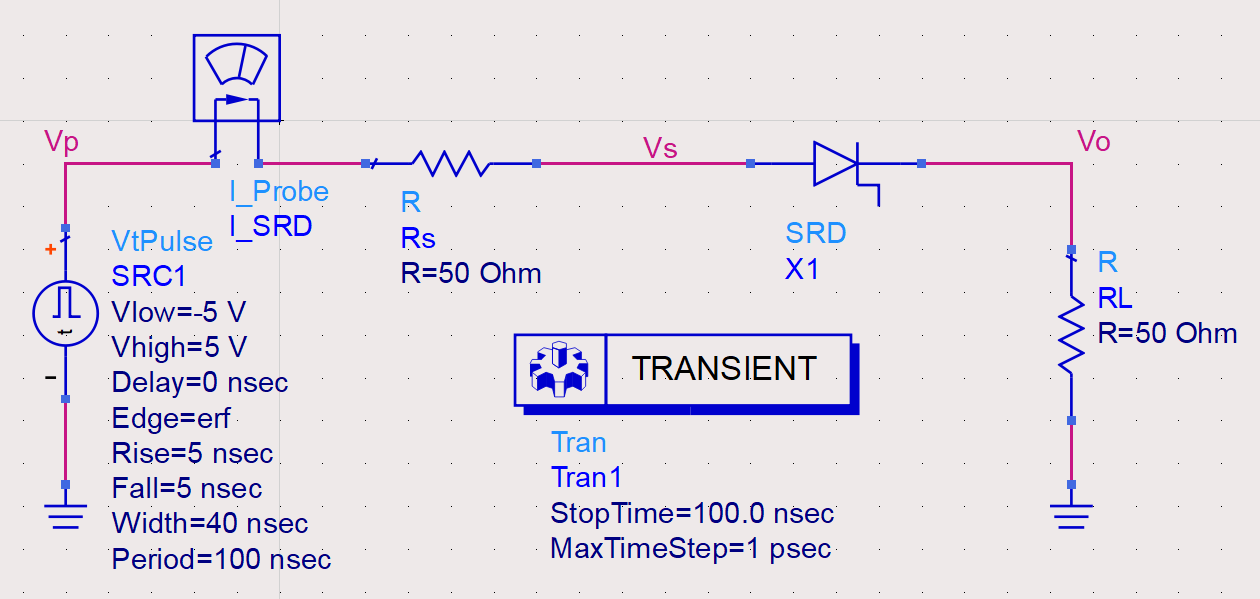
\includegraphics[width=0.6\textwidth]{images/srd_sharpener_circuit.png}
    \caption{Circuito afilador de flanco con SRD}
    \label{fig:srd_sharpener}
\end{figure}

El circuito está compuesto por un generador de cuadrada lento, con tiempos de
crecimiento y decrecimiento de \qty{5}{\nano\second}, en serie una resistencia
de fuente $R_s$ de valor \qty{50}{\ohm}. La carga del circuito es la resistencia
$R_L$ de \qty{50}{\ohm}.

\begin{figure}[tbp]
    \centering
    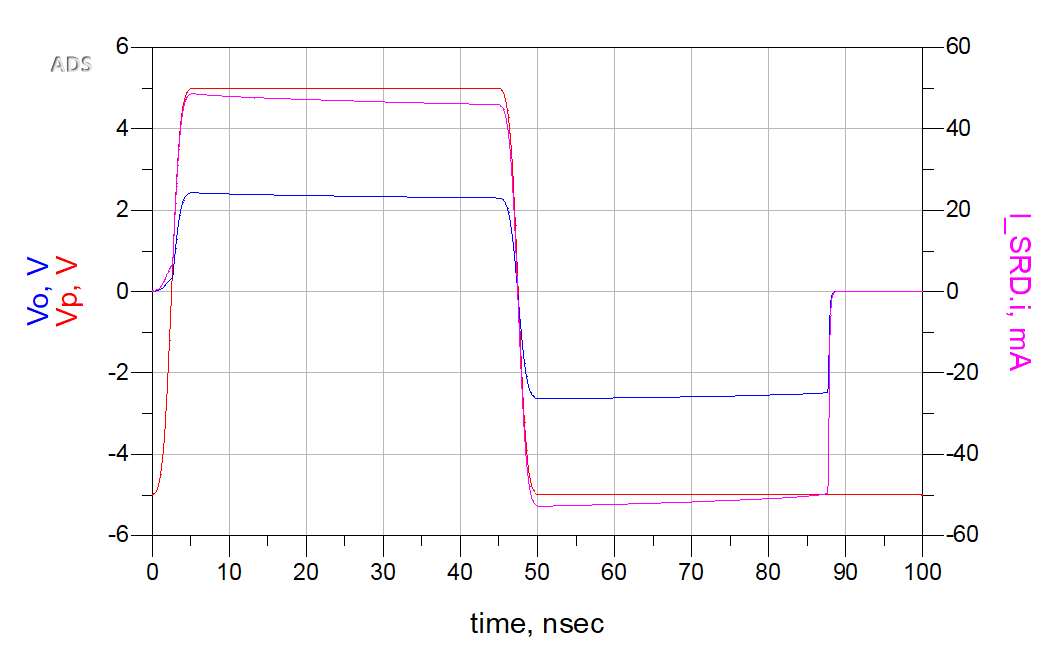
\includegraphics[width=0.8\textwidth]{images/srd_sharpener_result.png}
    \caption{Resultado de simulación.}
    \label{fig:srd_sharpener_result}
\end{figure}

En la figura \ref{fig:srd_sharpener_result} se observa el resultado de la
simulación. Vemos que, hasta aproximadamente \qty{85}{\nano\second}, la señal de
salida $V_o$ es igual a la señal de entrada, afectada por el divisor entre $R_L$
y $R_s$, $\frac{R_L}{R_L+R_s}$. Durante este tiempo, el \textit{SRD} presenta
una baja impedancia. En la porción positiva de la señal de entrada $V_p$, esto
es coincidente con un diodo usual, ya que el mismo se encuentra polarizado en
directa. En lo que destaca el \textit{SRD} de un diodo usual, es que luego de que la
tensión de entrada se invierta, este sigue presentando una baja impedancia. Esto
se debe al gran tiempo de vida de sus portadores minoritarios, lo que requiere
un tiempo apreciable para descargarlos y pasar al estado de alta impedancia.

Se observa en la forma de onda de $V_o$ que esta transición se da alrededor de
\qty{85}{\nano\second}, done la tensión de salida cae abruptamente a $0$. En la
figura \ref{fig:srd_sharpener_result} puede observarse el comportamiento
de la corriente. Se observa la misma caída abrupta en los
\qty{85}{\nano\second}, y una inversión en el signo de la corriente con la
inversión en el signo de la cuadrada de entrada.

\begin{figure}[tbp]
    \centering
    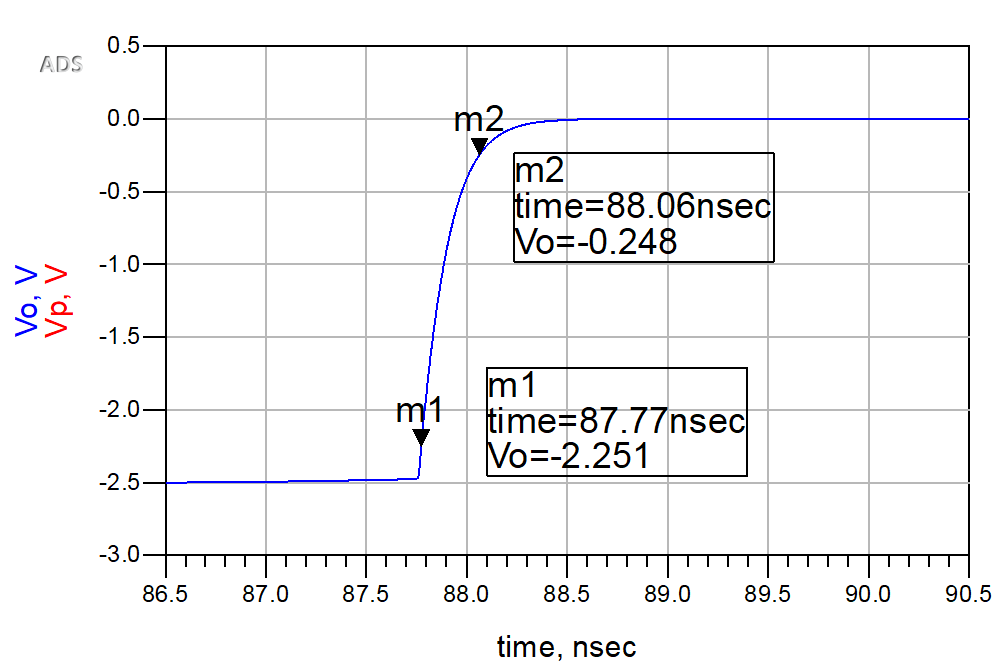
\includegraphics[width=0.8\textwidth]{images/srd_sharpener_result_rise_time.png}
    \caption{Tiempo de crecimiento.}
    \label{fig:srd_sharpener_result_rise_time}
\end{figure}

Llamaremos corriente de inyección de carga $I_F$ a la corriente que circula por
el \textit{SRD} con sentido positivo. Esta corriente determina la carga
almacenada en el mismo, y ambas se relacionan mediante \cite{an918},
\cite{moll1969}

\begin{equation}
    Q_F = I_F \cdot \tau \cdot \left( 1 - e^{-t_F/\tau}\right)
\end{equation}

Para el circuito presentado, la corriente $I_F$ estará dada por

\begin{equation}
    I_{F} = \frac{V_h}{R_s+R_L}
\end{equation}

con $V_h$ el valor de la tensión positiva de la señal cuadrada de entrada.

Para la corriente de extracción de carga $I_R$, que es la corriente que extrae
carga durante el tiempo en el que el \textit{SRD} se encuentra en un estado de
baja impedancia y la corriente que circula es negativa, tenemos la siguiente
expresión

\begin{equation}
    I_{R} = \frac{V_l}{R_s+R_L}
\end{equation}

con $V_l$ el valor de la tensión negativa de la señal cuadrada de entrada.

En la figura \ref{fig:srd_sharpener_result_rise_time}, puede observarse el
tiempo de crecimiento del escalón generado con el apagado del \textit{SRD}. Se
toma el tiempo de crecimiento \qty{10}{\percent}-\qty{90}{\percent}. Siendo que
el escalón de tensión se da entre \qty{-2.5}{\volt} y \qty{0}{\volt}, tenemos
que el punto de \qty{10}{\percent} es $V_{10\%} = -2.5 \ V \ \cdot 0.9 =  2.25 \
V$, y el de \qty{90}{\percent} es $V_{90\%} = -2.5 \ V \ \cdot 0.1 =  -0.25 \
V$.

En cuanto a la magnitud del salto de tensión $\Delta V$, estará dado por el
valor de la tensión en el cátodo del \textit{SRD} antes de que pase al estado de
alta impedancia. Esta tensión estará dada por el divisor entre $R_L$ y $R_s$,

\begin{equation}
    \Delta V = V_l \cdot \frac{R_L}{R_L+R_s}
\end{equation}

El tiempo de crecimiento de este escalón estará dado por dos componentes: un
tiempo de transición del diodo SRD $t_t$, y un tiempo de carga $RC$ dado por el
tiempo en que demora en cargarse el RC. \textcolor{red}{COMPLETAR CON EXPRESIÓN}
\cite{an918}.

\textcolor{red}{EXPLICAR IMPORTANCIA DE BAJA CAPACIDAD PARALELO AL SRD}

Vemos por los marcadores de la figura, que estos tiempos son
\qty{87.77}{\nano\second} y \qty{88.06}{\nano\second} respectivamente, por lo
que tenemos un tiempo de crecimiento

\begin{equation}
    t_r = \qty{87.77}{\nano\second} - \qty{88.06}{\nano\second} =
    \qty{290}{\pico\second}
\end{equation}

Como fuese explicado en la sección \textcolor{red}{AGREGAR REF\ref{TODO}}, este
tiempo de crecimiento estará dado por el tiempo de transición del diodo y por el
tiempo del RC formado entre la capacidad de reversa del diodo y la resistencia
vista desde los nodos del capacitor.

\section{Generador de pulsos con \textit{stub}}
\label{sec:generador_pulsos_stub}

\subsection{Principios del \textit{stub}}

Un \textit{stub} consiste de una línea de transmsión conectada en paralelo al
camino de la señal. Su efecto sobre la señal dependerá de su impedancia
característica, largo e impedancia de terminación \cite{pozar2011}.

Cuando el \textit{stub} se encuentra abierto, es decir, terminado por una
impedancia infinita, la señal propagada se verá reflejada con signo positivo, y
en el caso de una línea de transmisión sin pérdidas, con un factor de ganancia
unitario. En el caso de una línea de transmisión real, las pérdidas resultaran
en un factor de atenuación. \textcolor{red}{chequear esto de la atenuación, y lo
q sigue de las aplicaciones de un stub abierto}.  Este efecto permite generar
resonancias en ciertas frecuencias, útiles para filtrado de señales o adaptación
de impedancias.

En el caso de un \textit{stub} cortocircuitado, es decir, con una impedancia de
terminación igual a $0$, el efecto será una reflexión de la señal con fase
opuesta, y un factor de atenuación dado por las pérdidas de la línea.

El caso de interés para el circuito generador de pulsos, es el del \textit{stub}
cortocircuitado, ya que la reflexión de señal con fase opuesta, permite generar
un pulso en base a una forma de onda creciente o decreciente.

\begin{figure}[tbp]
    \centering
    
\includegraphics[width=0.8\textwidth]{images/placeholder.jpg}
    \caption{Reflexiones en un \textit{stub} cortocircuitado.}
    \label{fig:stub_time_domain_waveforms}
\end{figure}

En la figura \ref{fig:stub_time_domain_waveforms} se observa el principio de
funcionamiento. Se observa un pulso de entrada, formado por una forma de onda de
tipo escalón, en nuestro caso este escalón será el mismo que en la figura
\ref{srd_sharpener_result_rise_time}. Este escalón se ve reflejado con polaridad
opuesta, y se suma al escalón de entrada.

Dado el tiempo de propagación de la línea de transmisión $T$, vemos que el
tiempo que tarda el pulso de entrada en reflejarse es $2*T$, el tiempo de un
camino de ida y vuelta. Dado que el pulso se forma cuando vuelve la componente
reflejada, vemos que el ancho de pulso estará dado por $2*T$. De esta forma, la
duración temporal del pulso y, por lo tanto, el ancho de banda del sistema,
estará dado por la longitud $L$ del \textit{stub}.

El tiempo de propagación $T$ está dado por la velocidad de propagación en la
línea de transmisión $v_p$ y el largo de la línea $L$.

En un medio con permisividad relativa $\kappa$ y permeabilidad magnética
relativa unitaria, la velocidad de propagación está dada por \cite{pozar2011}

\begin{equation}
  v_p = \frac{c_0}{\sqrt{\kappa}}
\end{equation}

Para una línea de transmisión, es posible desarrollar una \textit{permisividad
relativa efectiva} $\kappa_{eff}$, que es una función de la geometría de la
línea y sus materiales \cite{pozar2011}. Esta función puede obtenerse a través
de una forma cerrada, generalmente involucrando diversas aproximaciones, o
mediante métodos numéricos iterativos. El punto a resaltar es que, dada una
determinada estructura de línea de transmisión y sus materiales, se puede
considerar a $\kappa_{eff}$ una constante del circuito.

Es interesante notar que $\kappa_{eff}$ es una función del corte transversal de
la línea de transmisión, y no de su dimensión longitudinal. De esta manera,
$\kappa_{eff}$ es independiente del largo $L$ de la línea \cite{pozar2011}.

Entonces, el ancho de pulso $T_p$ está dado por

\begin{equation}
    T_p = 2 \cdot T = 2 \cdot \frac{L}{v_p} =2 \cdot \sqrt{\kappa_{eff}} \cdot \frac{L}{c_0}
\end{equation}

De esta forma, se puede diseñar el largo de línea $L$ para obtener un ancho de
pulso $T_p$ deseado

\begin{equation}
    \label{eq:stub_length_vs_delay}
    L = \frac{T_p}{2} \cdot \frac{c_0}{\sqrt{\kappa_{eff}}}
\end{equation}

De esta manera, el largo $L$ queda determinado por el ancho de pulso deseado
$T_p$ y la constante de propagación de la línea de transmisión utilizada
$\kappa_{eff}$.

\subsection{Generador de pulsos SRD+\textit{stub}}

Agregando un \textit{stub} cortocircuitado al afilador de flancos SRD
descripto anteriormente, podemos formar un generador de pulsos ultracortos. El
SRD genera un flanco rápido, y este flanco es convertido en un pulso
mediante la reflexión con fase opuesta en el \textit{stub}. 

El ancho de pulso es controlado por el largo del \textit{stub} como fuese
explicado anteriormente. La amplitud por la amplitud de la fuente, la relación
entra la impedancia de carga $Z_L$ y la del generador $Z_g$ y por el largo del
stub.

Como fuese explicado en secciones anteriores \textcolor{red}{EXPLICAR EN QUÉ
SECCIÓN}, el escalón de tensión generado en el SRD tiene una magnitud dada por

\begin{equation}
    \Delta V = V_l \cdot \frac{R_L}{R_L+R_s}
\end{equation}

El ancho del pulso, estará dado por el valor de este escalón en el instante en
el que el pulso reflejado se recombina, como puede observarse en la figura
\textcolor{red}{FIGURA MOSTRANDO REFLEXIÓN STUB}. Si asumimos que el escalón
crece como un sistema de primer orden con constante de tiempo $\tau$, el valor
del escalón en función del tiempo es

\begin{equation}
  V(t) = \Delta V \left( 1-e^{-\frac{t}{\tau}}\right)
\end{equation}

Siendo el tiempo que tarda el pulso en reflejarse ida y vuelta $2T$ o $T_p$, la
amplitud del pulso estará dada por

\begin{equation}
    \label{eq:A_p}
    A_p = V(2T) = V_l \cdot \frac{R_L}{R_L+R_s} \left( 1-e^{-\frac{2T}{\tau}}\right)
\end{equation}

Vemos que $\Delta V$ es el máximo valor que puede alcanzar el pulso, siendo la
relación $\frac{2T}{\tau}$ la que determina que porcentaje de este valor tomará
el pulso. Para $ \tau \ll T $, será $e^{-\frac{2T}{\tau}} \approx 1$, y por lo
tanto $A_p \approx 0$. Este es el mismo resultado que intuitivamente se
obtendría, que para señales con una variación temporal $\tau$ mucho menor al
tiempo de propagación en el \textit{stub} $T$, la señal será filtrada por el
efecto de puesto a tierra.

Para el caso de la señal de escalón generada por el SRD, es fácil obtener un
tiempo de crecimiento del orden de los cientos de picosegundos, por lo que su
amplitud resulta un porcentaje considerable de $\Delta V$. Cuanto más rápido sea
el flanco, mayor amplitud.

En la figura \ref{fig:stub_generator_circuit} podemos observar un esquemático
del generador de pulsos basado en SRD y \textit{stub}. La fuente es simétrica,
con amplitudes de \qty{\pm 5}{\volt}. La impedancia de fuente $Z_g$ se encuentra
perfectamente adaptada a la de carga $Z_L$, siendo ambas de \qty{50}{\ohm}. La
línea de transmisión es ideal, caracterizada únicamente por su impedancia
característica, \qty{50}{\ohm} en este caso, y su retardo de propagación,
\qty{60}{\pico\second} en este caso.

\begin{figure}[tbp]
    \centering
    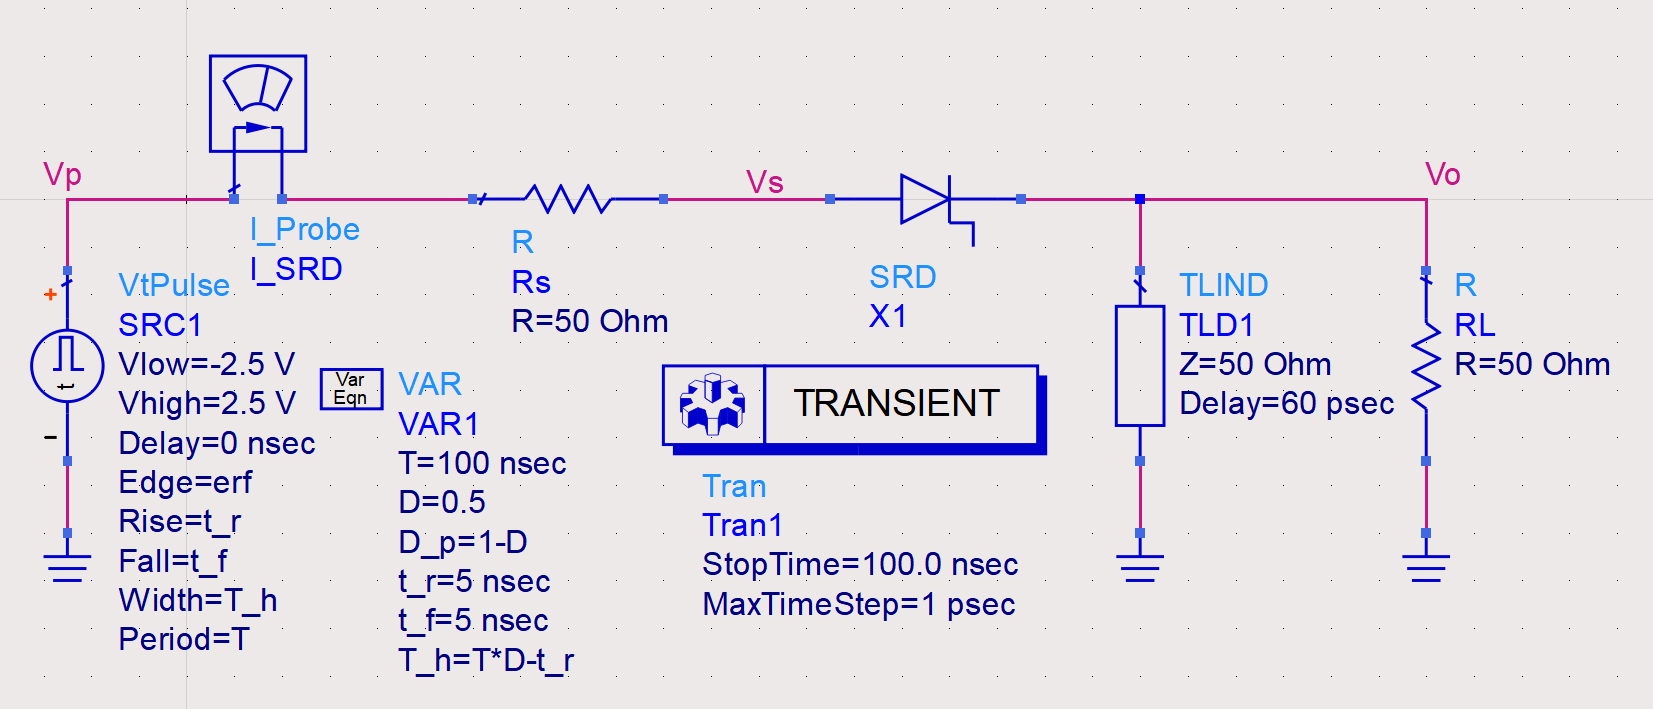
\includegraphics[width=0.8\textwidth]{images/stub_generator_circuit.png}
    \caption{Generador de pulsos basado en \textit{stub}}
    \label{fig:stub_generator_circuit}
\end{figure}

En la figura \ref{fig:stub_generator_sim_result} se observan los resultados de
la simulación del esquemático de la figura \ref{fig:stub_generator_circuit}. En
la figura  se observan las formas de onda de la señal de entrada $V_p$, la
tensión de salida $V_o$ y la corriente sobre el SRD $I_{SRD}$. Se observa que la
tensión de salida $V_o$ sigue a la de entrada $V_p$ hasta aproximadamente
\qty{85}{\nano\second}, donde el SRD pasa del estado de baja impedancia al de
alta. En en este instante, se forma un pulso por una combinación del salto de
tensión en el SRD y el efecto de reflexión del stub cortocircuitado. Es
interesante notar que los flancos positivos y negativos de la señal de entrada
también resultan en pulsos a la salida, aunque de mucha menor amplitud. La forma
de onda de la corriente es coincidente con lo mencionado anteriormente, siendo
una versión escalada por la impedancia de la forma de onda de entrada $V_p$,
hasta los \qty{85}{\nano\second}, donde cae abruptamente a $0$ debido al cambio
de impedancia en el SRD.

Es interesante notar que en este caso, los valores de la corriente están dados
por $\frac{V_p}{R_s}$ y no $\frac{V_p}{R_s+R_L}$ como en la sección
\ref{sec:srd_sharpener}. Esto se debe a que el \textit{stub} actua como un
cortocircuito sobre $R_L$, anulando su impedancia. Es importante notar que,
entonces, $R_S$ tiene la función de limitación de corriente durante las etapas
de conducción del SRD. De ser $0$ esta impedancia, la corriente sería infinita
(en rigor, se vería limitada únicamente por la resistencia serie del SRD)

En la figura \ref{fig:stub_generator_sim_result} se observa un zoom sobre el
pulso obtenido. Tiene una amplitud de \qty{1.728}{\volt}, y una duración
de \qty{180}{\pico\second} \textcolor{red}{por qué no es 60*2=120?}
\textcolor{red}{verificar que la amplitud coincida con la expresión anterior}.
Se observa que el pulso presenta un sobretiro negativo, una no idealidad no
contemplada hasta ahora en el modelo presentado.

\textcolor{red}{Hablar sobre la falta de reflexiones en el stub por ser de 50
ohm, q es la impedancia q ve una vez q se abre el SRD? ver q pasa si movemos esa
Zo?}

\begin{figure}[tbp]
    \centering
    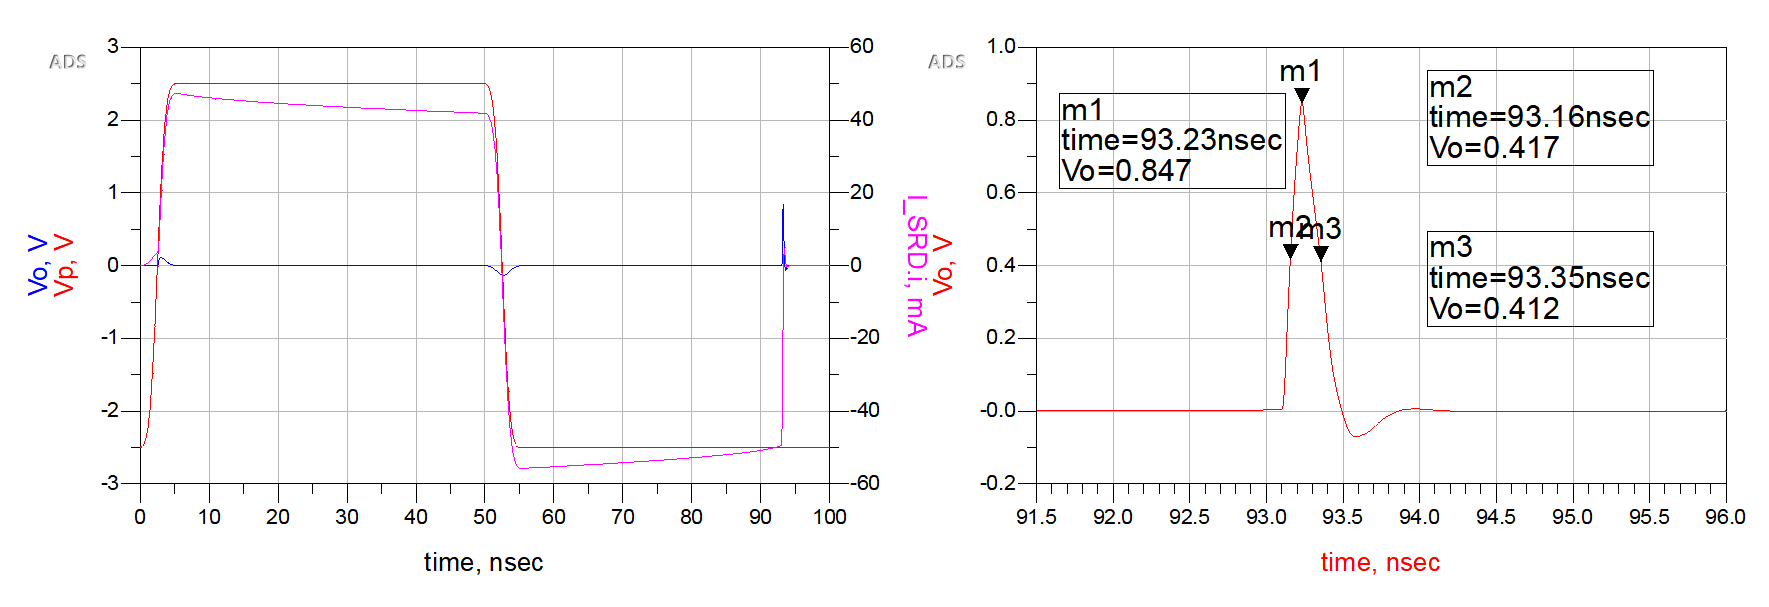
\includegraphics[width=0.8\textwidth]{images/stub_generator_sim_result.png}
    \caption{Resultado de simulación de generador con \textit{stub}}
    \label{fig:stub_generator_sim_result}
\end{figure}

\textcolor{red}{En algún lado calcular y simular el ancho de banda del pulso
generado}.

\section{Diseño final del \textit{pulser}}

Para compensar tanto las transmisiones de los flancos de la fuente de entrada y
el sobretiro negativo observado, se agrega al generador un diodo rectificador en
serie con la resistencia de carga $R_L$. Siendo la tensión de encendido del
diodo mayor a la amplitud de los pulsos generados por las transiciones de la
onda de entrada, estos no serán transmitidos a la carga $R_L$ debido a la acción
de rectificación. En cuanto al sobretiro, también será filtrado debido al
bloqueo de de corriente en sentido negativo.

Para un correcto funcionamiento del generador de pulsos, es fundamental que el
rectificador sea lo suficientemente rápido como para transmitir el pulso
ultracorto sin degradación. Por esta razón se utiliza un diodo Schottky.

El costo de este diodo es la perdida de amplitud en el pulso principal, dada por
la magnitud de su tensión de encendido

Para esta función de rectificación, se utilizó un diodo Schottky MA4E2502H
\cite{MA4E2502H-datasheet}. Este diodo con aplicaciones en rango de frecuencias
de microondas posee una muy baja capacidad total, del orden de
\qty{0.1}{\pico\farad}, y capacidad e inductancia parásitas extremadamente bajas
debido a su encapsulado. Esto permite trabajar en el ancho de banda necesario.
Además el encapsulado es de montaje superficial, por lo que es fácilmente
integrable. Su tensión de encendido es de \qty{650}{\milli\volt}, por lo que la
amplitud perdida se encontrará en ese orden.

\subsection{Simulaciones}

En la figura \ref{fig:pulser_w_schottky_sch} se observa un esquemático del
generador de pulsos con el rectificador incluido. En la figura
\ref{fig:pulser_w_schottky_sim_result} se observa el resultado de la
simulación. Para este caso, en la salida se encuentra únicamente el pulso
principal, habiéndose anulados los pulsos generados por las transiciones de la
señal de entrada.

En la figura \ref{fig:schottky_generator_result_pulse} se observa el pulso
simulado. Con respecto al de la simulación sin rectificador, figura
\ref{fig:stub_generator_sim_result}, se observa una perdida en la amplitud pico de
\qty{400}{\milli\volt}, dada por la tensión de encendido del Schottky
utilizado, y una anulación del sobretiro negativo.

\begin{figure}[tbp]
    \centering
    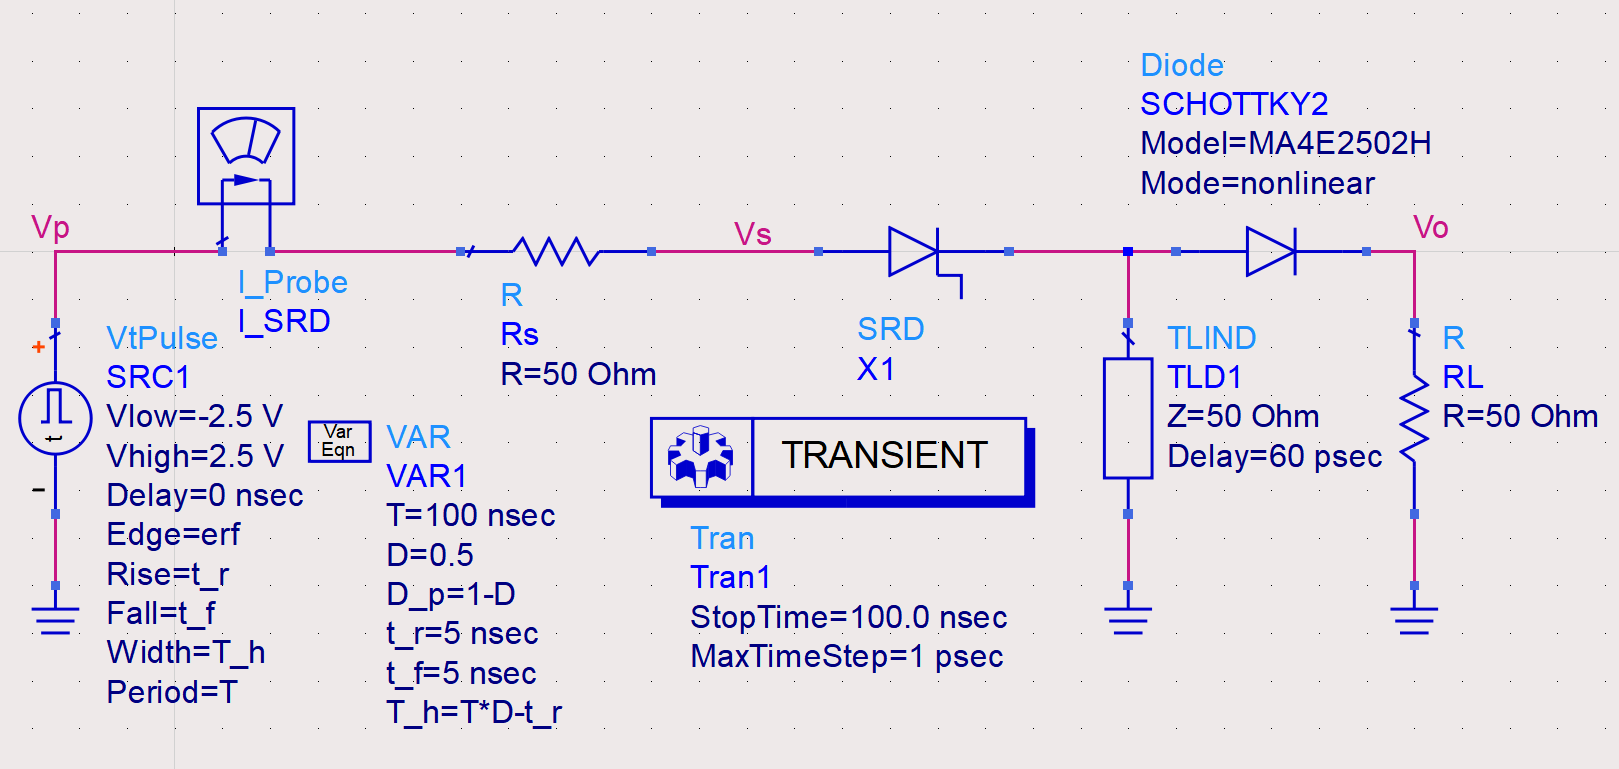
\includegraphics[width=0.8\textwidth]{images/pulser_w_schottky_sch.png}
    \caption{\textit{Pulser} final incluyendo diodo Schottky}
    \label{fig:pulser_w_schottky_sch}
\end{figure}

\begin{figure}[tbp]
    \centering
    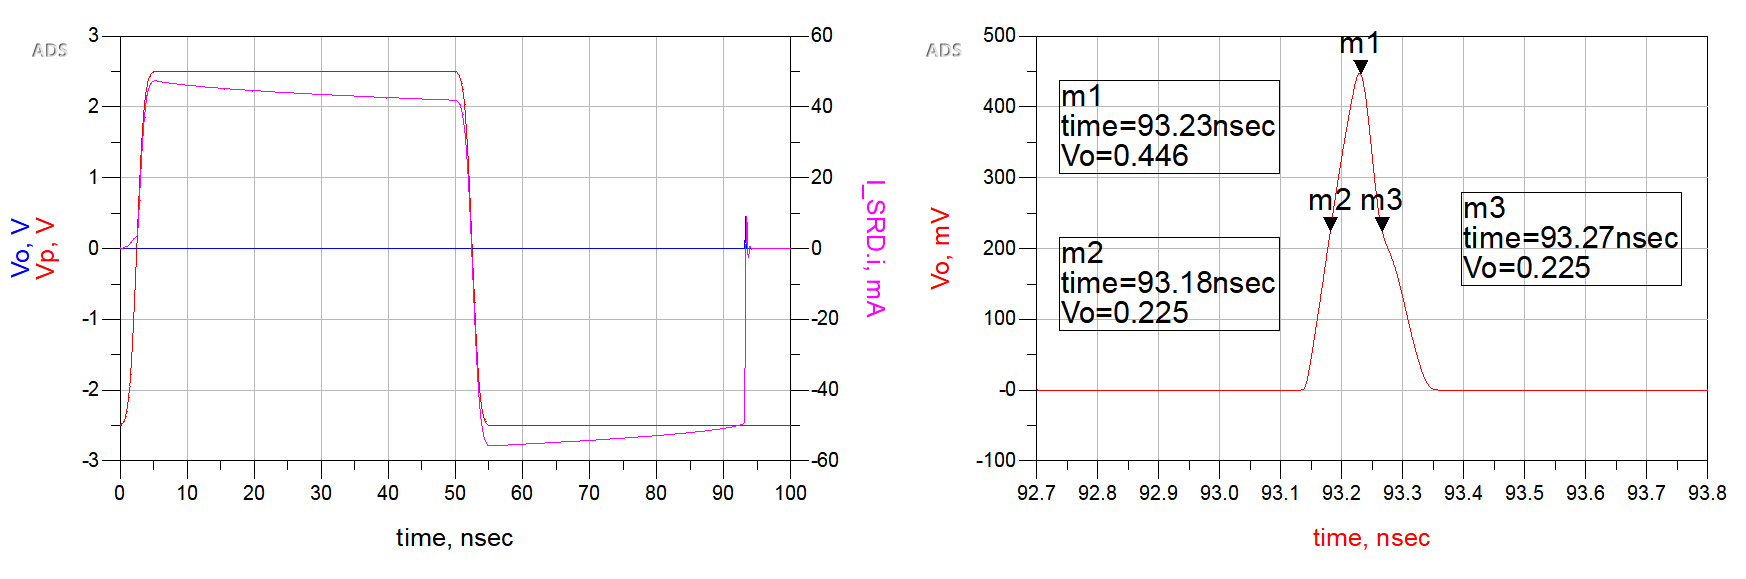
\includegraphics[width=0.8\textwidth]{images/pulser_w_schottky_sim_result.png}
    \caption{Resultado de simulación de generador con rectificador}
    \label{fig:pulser_w_schottky_sim_result}
\end{figure}

\section{Consumo del generador}
\label{sec:pulser_power}

El pulser final, que puede observarse en la captura del esquemático simulado en
la figura \ref{fig:stub_generator_circuit}, está compuesto por 3 componentes: la
resistencia serie $R_s$, el diodo SRD y el diodo Schottky. Calcularemos el
consumo de potencia de los 3.

Para un período de la señal cuadrada de entrada, podemos identificar 3 secciones

\begin{itemize}
    \item La sección positiva, en la que la tensión de la señal de entrada es
        positiva, y la corriente la aproximaremos constante y positiva.
    \item La sección de conducción negativa, en la que la tensión de la señal de
        entrada se vuelve negativa, y la corriente es constante y también
        negativa.
    \item La sección de no conducción, en la que la señal de entrada es
        negativa y ya no circula corriente debido a la transición al estado de
        alta impedancia del SRD.
\end{itemize}

La corriente en el SRD y $R_s$ durante un período de la señal cuadrada tendrá 3
valores: $I_+$ en el período positivo, $I_-$ en el de conducción negativa y $0$
en la sección de no conducción. La corriente RMS es

\begin{equation}
    \begin{aligned}
        I_{RMS}^2 &= \frac{1}{T} \cdot \int_{t_0}^{t_0+T} i(t)^2dt = \frac{1}{T}
        \cdot \left( D \cdot T \cdot I_+^2 + T_s \cdot I_-^2 \right) \\
        I_{RMS}^2 &= D \cdot I_+^2 + \frac{T_s}{T} \cdot I_-^2 \\
        I_{RMS}^2 &< D \cdot I_+^2 + D' \cdot I_-^2 \\
    \end{aligned}
\end{equation}

Podemos acotar a la corriente RMS con $D \cdot I_+^2 + D' \cdot I_-^2$.
Despreciando la caída de tensión en el SRD, las expresiones de estas corrientes son

\begin{equation}
    \begin{aligned}
        I_+ &= \frac{V_+}{R_s} \\
        I_- &= \frac{V_-}{R_s} \\
    \end{aligned}
\end{equation}

Tomando como tensión máxima \qty{10}{\volt}, tenemos que la corriente máxima será
$I_M = \qty{200}{\milli\ampere}$.

\begin{equation}
    \begin{aligned}
        I_{RMS}^2 &< D \cdot \left( \frac{V_+}{R_s} \right) ^2 + D' \cdot
        \left( \frac{V_-}{R_s} \right) ^2 \\
        I_{RMS}^2 &< D \cdot \left( \frac{\qty{10}{\volt}}{\qty{50}{\ohm}} \right) ^2 + D' \cdot
        \left( \frac{\qty{10}{\volt}}{\qty{50}{\ohm}} \right) ^2 \\
        I_{RMS}^2 &< \left( \frac{\qty{10}{\volt}}{\qty{50}{\ohm}} \right) ^2  \\
        I_{RMS} &< \qty{200}{\milli\ampere} \\
    \end{aligned}
\end{equation}

En cuanto a la corriente de la rama de salida, esta está será igual a

\begin{equation}
    i_o(t) = \frac{v_o(t)}{R_L}
\end{equation}

Podemos acotar el consumo tomando un pulso de peor caso de \qty{3}{\volt} de
amplitud y \qty{0.5}{\nano\second} de duración.

\begin{equation}
    \begin{aligned}
        V_{RMS}^2 &< \frac{1}{T} \cdot \int_{t_0}^{t_0+T} v(t)^2dt =
        \frac{1}{\qty{100}{\nano\second}} \cdot \qty{0.5}{\nano\second} \cdot
        \left( \cdot \qty{3}{\volt} \right )^2 \\
        V_{RMS} &< \frac{\qty{3}{\volt}}{\sqrt{200}} \\
        V_{RMS} &< \qty{213}{\milli\volt}
    \end{aligned}
\end{equation}

En la impedancia de salida $Z_o$, esto resulta en una disipación de potencia

\begin{equation}
    \begin{aligned}
        P_{o} &= \frac{V_{RMS}^2}{R_o} \\
        P_{o} &= \frac{ \qty{213}{\milli\volt}^2}{ \qty{50}{\ohm}} \\
        P_{o} &= \qty{0.3}{\milli\watt} \\
    \end{aligned}
\end{equation}

Que representa una potencia prácticamente despreciable.

En el caso del diodo Schottky, asumiendo una tensión de encendido constante
durante la duración del pulso y de un valor igual a \qty{650}{\milli\volt},
tenemos

\begin{equation}
    \begin{aligned}
        P_{D} &< \frac{1}{T} \cdot \int_{t_0}^{t_0+T} v(t) \cdot i(t) dt =
        \frac{1}{T} \cdot \int_{t_0}^{t_0+T} V_D \cdot \frac{v_o(t)}{R_o} dt \\
        P_{D} &< \frac{1}{\qty{100}{\nano\second}} \cdot \left( \qty{0.5}{\nano\second} \cdot
        \qty{650}{\milli\volt} \cdot \frac{\qty{3}{\volt}}{
            \qty{50}{\ohm}} \right) \\
        P_{D} &< \qty{0.2}{\milli\watt} \\
    \end{aligned}
\end{equation}

La máxima potencia especificada por el fabricante es de \qty{50}{\milli\watt},
por lo que nos encontramos muy por debajo del límite.

\section{Diseño del \textit{driver}}

Dado que uno de los objetivos del trabajo es un generador de pulsos que pueda
ser controlado por la salida digital de un sistema embebido, y dado que estas
salidas son en la mayoría de los casos unipolares y de baja capacidad de carga,
es necesario incluir en el prototipo una etapa \textit{driver}.

La función de esta etapa es, en base a un pulso digital de entrada de control, y
una fuente de alimentación continua, generar el pulso bipolar necesario para el
funcionamiento del \textit{pulser}. Este pulso bipolar tendrá un ciclo de
trabajo y un período dados por el ciclo de trabajo y el período del pulso
unipolar de entrada. Es necesario también que el \textit{driver} presente una
baja carga al pulso unipolar.

En la figura \ref{fig:driver_block_diagram} se observa un diagrama en bloques
del driver propuesto. El mismo está compuesto por dos componentes principales
que brindan dos funciones diferenciadas, la llave y el capacitor. A la entrada
es excitado por la señal digital de control, y a la salida tiene una carga
$Z_L$. La carga en este caso será el pulser, por lo tanto será una carga no
lineal, ya que como se mostró en secciones anteriores, la corriente que consume
tiene una abrupta caída a 0 cuando se abre el SRD.

\begin{figure}[tbp]
    \centering
    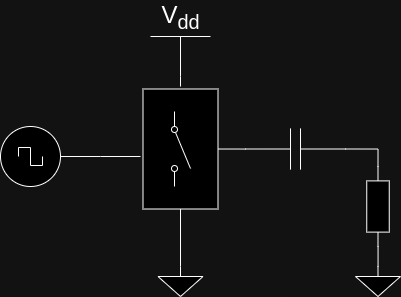
\includegraphics[width=0.8\textwidth]{images/driver.drawio.png}
    \caption{Diagrama en bloques del driver}
    \label{fig:driver_block_diagram}
\end{figure}

La llave conmuta entre $V_{dd}$ y tierra según la señal de control digital. De
esta manera, la corriente que consume la carga es entregada por la fuente y no
por la señal de control digital. A la salida de la llave se generará una señal
cuadrada unipolar, pero a diferencia de la entrada, esta conmutará entre
$V_{dd}$ y tierra, mientras que a la entrada se conmuta entre $V_{dig}$ y
tierra. De esta manera, la llave logra presentarle una carga baja y constante a
la salida digital, y amplifica la conmutación a todo el rango disponible con la
fuente de alimentación. Esta es una aproximación ideal, en realidad será todo el
rango de la fuente de alimentación menos la caída que tenga el bloque.

A la salida de la llave tenemos entonces una señal cuadrada unipolar, con
amplitud pico a pico igual a $V_{dd}$, es decir, toda la amplitud disponible de
la fuente de alimentación, y una capacidad de entrega de corriente considerable.
Para convertir esta señal en una bipolar, se utiliza un filtro pasa altos, que
elimina la componente continua de la señal unipolar, resultando en una bipolar.

En las próximas secciones se explica en detalle los requerimientos e
implementación de cada uno de estos bloques.

\subsection{Filtro pasa altos}

Sabemos que un pulso cuadrado unipolar de período $T$ tendrá un espectro dado
por una componente de continua con el valor medio $V_{m}$, y múltiples
harmónicos de $T$, cada uno con una amplitud que decae con $\frac{1}{n}$.
\textcolor{red}{agregar una referencia que banque esto}.

Entonces, podemos pensar al pulso unipolar como la suma de un pulso bipolar de
valor medio 0, y una constante con valor igual al valor medio del pulso
unipolar. Entonces, podemos obtener al pulso bipolar restándole al unipolar su
valor medio.

Teniendo en cuenta que el valor medio es la componente de DC del pulso, podemos
lograr este resultado pasando el pulso unipolar por un filtro pasa altos. El ancho
de banda de este filtro debe ser tal que filtre la componente de continua y no
distorsione las componentes alternas, que se encuentran a partir de $T$.

Sabemos que un filtro pasa altos de primer orden con frecuencia de corte $f_c$
tiene una característica de magnitud que presenta atenuación desde continua hasta
aproximadamente $f_c$, y una fase que varía \qty{90}{\degree} desde
$\frac{f_c}{10}$ hasta $f_c \cdot 10$. Entonces, para filtrar la componente
continua de la unipolar y transmitir la bipolar sin distorsión,
es necesario que la frecuencia de la cuadrada sea mayor a 10 veces $f_c$, es
decir $T > 10 \cdot f_c$, o $f_c < \frac{T}{10}$.

Siendo la $PRF$ objetivo de \qty{10}{\mega\hertz}, el requerimiento sobre $f_c$
es entonces $f_c < \qty{1}{\mega\hertz}$.

Para implementar el filtro pasa altos propuesto, se optó por un filtro de primer
orden RC. Para lograr la característica pasa altos, el capacitor debe estar en
el camino de la señal, es decir, en serie. De esta manera, el filtro queda
compuesto por un capacitor $C$ serie y una impedancia $Z$ dada por la impedancia
de entrada del pulser, asumiendo una impedancia despreciable para la llave.

Para una estimación del rango de valores posibles para $C$ asumimos un rango
para $Z$ de $ Z \approx \qty{50}{\ohm}$. Esta es una aproximación razonable dado
que el sistema trabaja en \qty{50}{\ohm}, por lo que $Z$ será una serie de
impedancias cercanas a \qty{50}{\ohm} en serie o paralelo, lo que resultará en
una impedancia en ese mismo orden de valores. De esta manera,

\begin{equation}
    \begin{aligned}
        f_c &< \qty{1}{\mega\hertz} \\
        \frac{1}{2\pi \cdot |Z| \cdot C} &< \qty{1}{\mega\hertz} \\
        C &> \frac{1}{2\pi \cdot |Z| \cdot \qty{1}{\mega\hertz}} \\
        C &> \frac{1}{2\pi \cdot \qty{50}{\mega\hertz} \cdot \qty{1}{\mega\hertz}} \\
        C &> \qty{3.2}{\nano\farad} \\
    \end{aligned}
\end{equation}

La capacidad debe estar por arriba de \qty{3.2}{\nano\farad}, valores fácilmente
obtenibles en los tamaños de encapsulados objetivo.

\textcolor{red}{explicar q vamos incluso más arriba de esto para q la tensión en
el capacitor sea constante y no una triangular}

En la siguiente sección, asumiendo un filtrado ideal, es decir, donde se filtra
por completo el valor medio $V_m$ y se transmiten los harmónicos sin distorsión,
se desarrolla la expresión de los valores de la bipolar.

\subsubsection{Cuadrada unipolar filtrada por pasa altos}

El valor medio de la tensión $V_m$ en una señal cuadrada con valores $V_+$ y
$V_-$, con período $T$ y ciclo de trabajo $D$ está dado por

\begin{equation}
    V_m = D \cdot V_+ + (1-D) \cdot V_-
\end{equation}

En nuestro caso, la señal unipolar a la salida de la llave tiene valores
$V_+=V_{dd}$ y $V_-=0$, por lo que tiene un valor medio

\begin{equation}
    V_m = D \cdot V_{dd}
\end{equation}

La cuadrada desarrollada en la impedancia de carga $Z_L$ será la cuadrada
unipolar a la salida de la llave, menos su valor medio. Esta señal tendrá
entonces valores $V_+$ y $V_-$ dados por

\begin{equation}
    \label{eq:square_linear_load_highpassed_values}
    \begin{aligned}
        V_+ &= V_{dd}-V_m = V_{dd} \cdot (1-D) \\
        V_- &= -V_m = -V_{dd} \cdot D \\
    \end{aligned}
\end{equation}

Estos son los valores de la señal cuadrada unipolar que excitará al pulser.
Entonces, reconocemos que $V_-$ es $V_l$ en la ecuación \ref{eq:A_p}.

\begin{equation}
    A_p = V_{dd} \cdot D \cdot \frac{R_L}{R_L+R_s} \left( 1-e^{-\frac{2T}{\tau}}\right)
\end{equation}

Entonces, tanto el valor absoluto de $V_{dd}$ como el valor de $D$ incrementan
linealmente la amplitud del pulso a la salida. Aumentar $V_{dd}$ tiene como
límite la conducción de corriente máxima en los componentes del circuito,
mientras que $D$ tiene como límite superior el tiempo de descarga $T_s$,
teniendo que se ser $T*(1-D) > T_s$, es decir, el tiempo en el que la cuadrada
bipolar tiene el valor $V_l$ tiene que ser suficiente para la remoción de todas
las cargas en el SRD.

\subsubsection{Pasa altos con \textit{pulser}}
\label{sec:carga_no_lineal}

Simulamos el circuito pasa altos utilizando como carga al pulser. En la figura
\ref{fig:highpass_filter_nonlinear_load_sch} puede observarse el esquemático
simulado. A la entrada, tenemos una fuente unipolar de \qty{5}{\volt} de
amplitud, con un ciclo de trabajo $D=0.5$. En base a
\ref{eq:square_linear_load_highpassed_values}, esperamos en el nodo
$V_{bipolar}$ una señal cuadrada simétrica con amplitudes de
\qty{\pm2.5}{\volt}. Siendo la constante de tiempo del circuito pasa altos $\tau
\approx \qty{100}{\nano\farad} \cdot \qty{50}{\ohm} = \qty{5}{\micro\second}$,
el tiempo total de simulación es de \qty{50}{\micro\second} de manera tal de
capturar 10 constantes y analizar el estado permanente del circuito.

\begin{figure}[tbp]
    \centering
    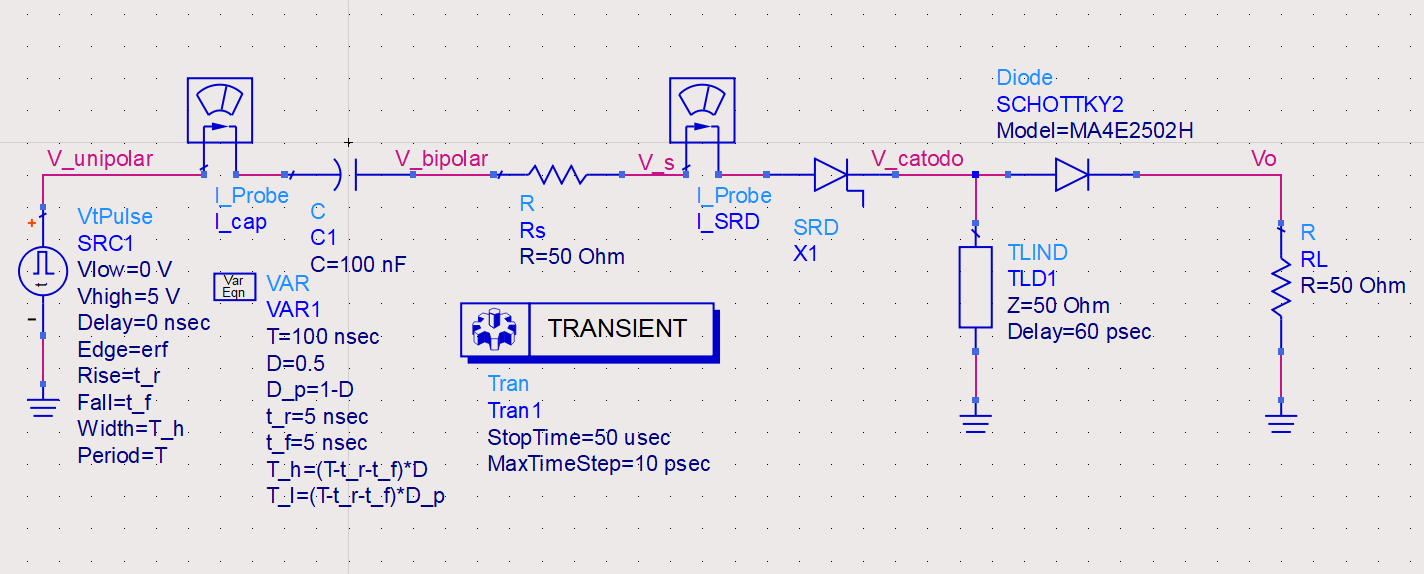
\includegraphics[width=0.99\textwidth]{images/highpass_filter_nonlinear_load_sch.png}
    \caption{Esquemático simulado para filtro pasa altos con carga no lineal.}
    \label{fig:highpass_filter_nonlinear_load_sch}
\end{figure}

\begin{figure}[tbp]
    \centering
    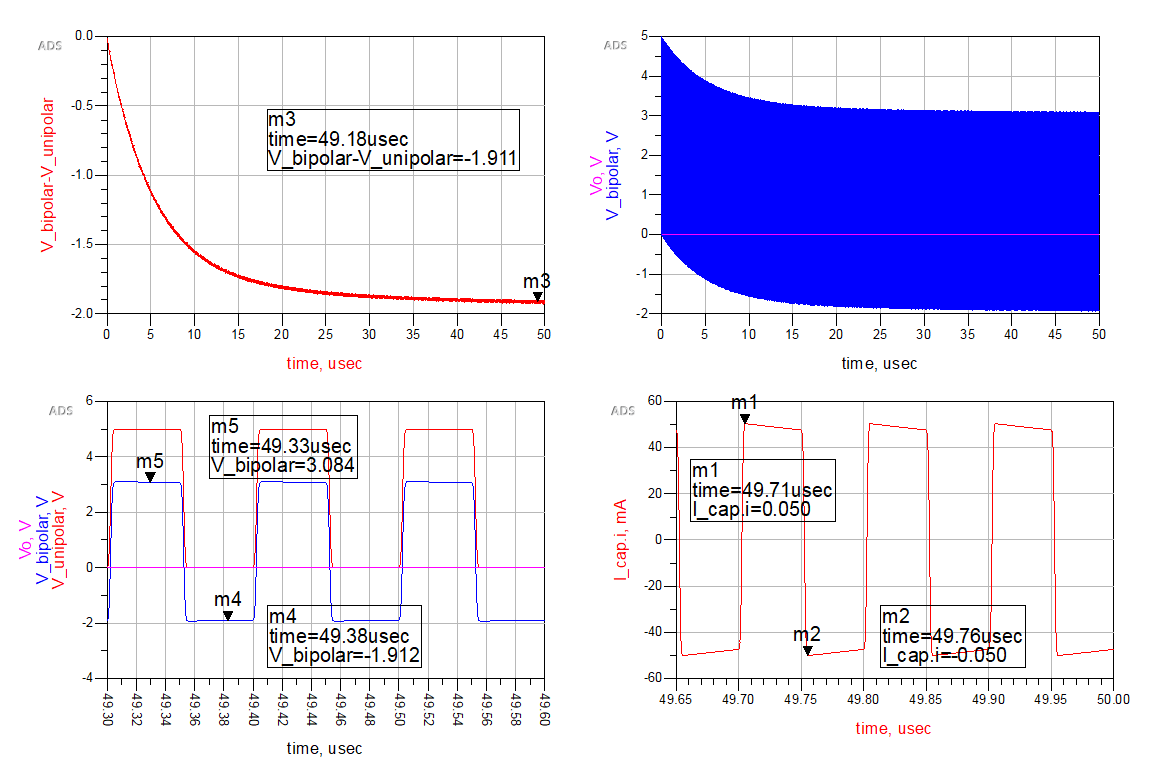
\includegraphics[width=0.99\textwidth]{images/highpass_filter_nonlinear_load_sim_result.png}
    \caption{Resultados de simulación para filtro pasa altos con carga no lineal.}
    \label{fig:highpass_filter_nonlinear_load_sim_result}
\end{figure}

En la figura \ref{fig:highpass_filter_nonlinear_load_sim_result} se observan los
resultados de la simulación. Contrario a lo predecido por
\ref{eq:square_linear_load_highpassed_values}, los valores de $V_{bipolar}$ no
son \qty{\pm2.5}{\volt}, sino \qty{3}{\volt} y \qty{-1.9}{\volt}. Esto es
consistente con el valor en estado estacionario de la tensión en el capacitor,
que es \qty{-1.9}{\volt}, y no \qty{-2.5}{\volt.}

En cuanto al nodo de salida $V_o$, vemos que no desarrolla los pulsos esperados,
y que encuentra constante en \qty{0}{\volt}. Esto es consistente con la forma de
onda bipolar generada: al presentar un nivel de tensión positivo de mayor
magnitud al negativo, aplicándose ambos niveles durante el mismo tiempo (es
decir $D=0.5$), es esperado que la carga inyectada al SRD no sea removida, no
pasando este al estado de alta impedancia y, por lo tanto, no se de la
generación de pulsos.

Esto se confirma observando la forma de onda de la corriente: es simétrica, con
la misma corriente siendo inyectada en la porción positiva de la cuadrada
bipolar que siendo removida en la porción negativa.

Desarrollaremos en detalle el comportamiento del filtro pasa altos con una carga
no lineal para explicar la razón de este problema, y presentar una solución al
mismo.

\subsubsection{Carga lineal}

Empezamos analizando el caso de una carga lineal, pero sin apelar a argumentos
de función transferencia, ya que para el caso de una carga no lineal no son
validos. Basaremos el análisis en el balance ampere-segundo en el capacitor
\cite{Erickson_Robert_W_2020}. Este resultado establece que el valor medio de la
corriente en un capacitor en estado estacionario es nulo.

\begin{equation}
    \label{eq:capacitor_ampere_second_balance}
    \langle i(t) \rangle = \int_{t_0}^{t_0+T} i(t)dt = 0
\end{equation}

En caso de una carga $Z_L$ lineal, la corriente y la tensión están linealmente
relacionadas, conduciendo al resultado de la sección anterior en el que tanto la
tensión como la corriente tienen un valor medio 0. En el caso de la carga no
lineal, se mantiene la ecuación \ref{eq:capacitor_ampere_second_balance}, es
decir, el valor medio de la corriente en el capacitor será cero, pero no
necesariamente el de la tensión será 0.

Asumiendo que en estado permanente el capacitor se carga a una tensión constante
$V_C$, este valor será el que resulte de imponer el cumplimiento de la ecuación
\ref{eq:capacitor_ampere_second_balance}.

\begin{figure}[h!]
    \begin{center}
        \begin{circuitikz}[american]
            \draw (0,3) to [V, l=$V_U$] (0,0)
            (0,3) to [C=$C$, v=$V_C$] (4,3)
            (4,3) to [R=$R$] (4,0) --
            (0,0);
        \end{circuitikz}
    \end{center}
    \caption{Circuito pasa altos con carga lineal}
    \label{fig:sch_highpass_non_linear_load}
\end{figure}

Para el caso de una carga lineal, tenemos un circuito como el de
\ref{fig:sch_highpass_non_linear_load}. Asumiendo que durante las porciones
positivas y negativas de la tensión unipolar tenemos corrientes constantes $I_+$
e $I_-$, aplicando \ref{eq:capacitor_ampere_second_balance} llegamos a 

\begin{equation}
    \label{eq:current_balance_capacitor_linear_load}
    \begin{aligned}
        \int_{t_0}^{t_0+T} i(t)dt &= I_+ \cdot D - I_- \cdot D' = 0 \\
        I_+ \cdot D &= I_- \cdot D' \\
    \end{aligned}
\end{equation}

En este caso, las corrientes son

\begin{equation}
    \label{eq:highpass_currents_linear_load}
    \begin{aligned}
        I_+ &= \frac{V_U-V_C}{R} \\
        I_- &= \frac{Vc}{R} \\
    \end{aligned}
\end{equation}

Reemplazando en \ref{eq:current_balance_capacitor_linear_load},

\begin{equation}
    \label{eq:vc_linear_load}
    \begin{aligned}
        \frac{V_U-V_C}{R} \cdot D &= \frac{Vc}{R} \cdot D' \\
        V_U \cdot D &= V_C \cdot \left( D'+D \right) \\
        V_C &= V_U \cdot D \\
    \end{aligned}
\end{equation}

Es el mismo resultado que en la sección anterior.

\subsubsection{Carga no lineal}

Ahora, supongamos una carga no lineal de las siguientes características: conduce
durante todo el período positivo de la unipolar $D$, y una porción $\alpha \cdot
D'$ de la porción negativa, con $\alpha \in \left[0, 1 \right]$. En la figura
\ref{fig:alpha_definition_plot} se muestra gráficamente la definición. Un
$\alpha=0$ corresponde a una carga que no conduce en la porción negativa, como
un diodo usual, y una de $\alpha=1$ corresponde a una carga lineal. En nuestro
caso, es $\alpha = 2 \cdot \frac{T_s}{T}$, con $T_s$ el tiempo de descarga del
SRD, es decir, el tiempo que le toma  a la corriente negativa extraer todas las
cargas inyectadas en la porción positiva.

\begin{figure}[h!]
    \begin{center}
        \begin{tikzpicture}
          \def\D{0.5}
          \def\Alpha{0.5}
          \def\Iplus{0.7}
          \def\Iminus{-1.2}

          \begin{axis}[
            xlabel=$t$,
            ylabel=$i$,
            xmin=0, xmax=1,
            ymin=\Iminus-1, ymax=\Iplus+1,
            samples=100,
            axis lines=center,
            xtick={0,\D,\D+(1-\D)*\Alpha},
            ytick={\Iminus,\Iplus},
            domain=0:1,
            xticklabels={$0$, $D \cdot T$, $\alpha \cdot D' \cdot T$},
            yticklabels={$I_{-}$, $I_{+}$},
          ]

          % Square wave function
          \def\sqwave(#1){
            ifthenelse(#1 < \D, \Iplus,
              ifthenelse(#1 < \D+\Alpha*(1-\D), \Iminus, 0))
          }

          \addplot[blue, thick, domain=0:1, samples=500] {\sqwave(x)};
          \end{axis}
        \end{tikzpicture}
    \end{center}
    \caption{Definición del parámetro $\alpha$}
    \label{fig:alpha_definition_plot}
\end{figure}
En este caso, el balance de corrientes es

\begin{equation}
    \label{eq:current_balance_capacitor_linear_load}
    \begin{aligned}
        \int_{t_0}^{t_0+T} i(t)dt &= I_+ \cdot D - I_- \cdot \alpha \cdot D' = 0 \\
        I_+ \cdot D &= I_- \cdot \alpha \cdot D' \\
    \end{aligned}
\end{equation}

Las corrientes $I_+$ e $I_-$ son las mismas que en
\ref{eq:highpass_currents_linear_load}. Entonces, llegamos a

\begin{equation}
    \label{eq:vc_non_linear_load_0}
    \begin{aligned}
        \frac{V_U-V_C}{R} \cdot D &= \frac{Vc}{R} \cdot \alpha \cdot D' \\
        V_U \cdot D &= V_C \cdot \left( \alpha \cdot D'+D \right) \\
        V_C &= V_U \cdot \frac{D}{\alpha \cdot D' + D}  \\
    \end{aligned}
\end{equation}

Definiendo a $\alpha'=\alpha-1$, tenemos

\begin{equation}
    \label{eq:vc_non_linear_load}
    \begin{aligned}
        \alpha \cdot D' &+ D \\
        (1-\alpha') \cdot D' &+ D \\
        \cdot D' - \alpha' \cdot D' &+ D \\
        1 - \alpha' \cdot D' & \\
    \end{aligned}
\end{equation}

Llegamos a

\begin{equation}
    \label{eq:vc_non_linear_load_final}
        V_C = V_U \cdot \frac{D}{1-\alpha' \cdot D}
\end{equation}

Vemos que para el caso de carga lineal $\alpha = 1 \ (\alpha'=0)$, la ecuación
se convierte en la misma que \ref{eq:vc_linear_load} como es esperado.

El resultado obtenido es consistente con el resultado de la simulación del pasa
altos con el pulser como carga. La ecuación
\ref{eq:vc_non_linear_load}  indica que a mayor $\alpha$, es decir, menor
conducción de corriente durante la porción negativa, menor es $V_C$, la tensión de
estado permanente en el capacitor. Este resultado es contrario a las necesidades
de operación del generador de pulsos, ya que este se basa en la transición al
estado de alta impedancia del SRD, es decir, en un $\alpha < 1$. Esta condición
resulta en un $V_C$ menor, lo que incrementa $I_+$ y decrementa $I_-$,
imposibilitando la remoción de carga en el SRD.

En la siguiente sección, desarrollamos el efecto de un resistor lineal en
paralelo con la carga no lineal. Se demostrará como este tiene el efecto de
linearizar la operación, compensando el efecto de $\alpha < 1$, y posibilitando
el funcionamiento del pulser.

\subsubsection{Carga no lineal en paralelo con carga lineal}

Tenemos un circuito como el de la figura
\ref{fig:circuit_non_linear_load_with_shunt}. Nombramos $R_s$ a la resistencia
de la rama no lineal, ya que en el caso del pulser, cuando la rama conduce, su
resistencia es igual a $R_s$. $R_{sh}$ es una resistencia propuesta para mitigar
el efecto mencionando anteriormente.

\begin{figure}[h!]
    \begin{center}
        \begin{circuitikz}[american]
            \draw (0,3) to [V, l=$V_U$] (0,0)
            (0,3) to [C=$C$, v=$V_C$] (4,3)
            (4,3) to [R=$R_{sh}$] (4,0)
            (4,3) to [spst] (6,3) --
            (6,3) to [R=$R_{s}$] (6,0) --
            (0,0);
        \end{circuitikz}
    \end{center}
    \caption{pasa altos con carga no lineal en paralelo con lineal}
    \label{fig:circuit_non_linear_load_with_shunt}
\end{figure}

Planteando el balance de corrientes en el capacitor, tenemos

\begin{equation}
    \label{eq:current_balance_capacitor_linear_load}
    \begin{aligned}
        \int_{t_0}^{t_0+T} i(t)dt &= \left( I_{+L} + I_{+NL} \right) \cdot D -
        \left( I_{-L} \cdot \cdot D' + I_{-NL} \cdot \alpha \cdot D'
        \right) = 0 \\
        \left( I_{+L} + I_{+NL} \right) \cdot D &= \left( I_{-L} + I_{-NL} \cdot
        \alpha \right) \cdot D' \\
    \end{aligned}
\end{equation}

Siendo ambas expresiones $I_{\pm-L}$ e $I_{\pm-NL}$ las de
\ref{eq:highpass_currents_linear_load} evaluando $R=R_{sh}$ y $R=R_{s}$
respectivamente, llegamos a

\begin{equation}
    \label{eq:vc_non_linear_load_with_shunt_0}
    \begin{aligned}
        \left( \frac{V_U-V_C}{R_{sh}} + \frac{V_U-V_C}{R_{s}} \right) \cdot D &=
        \left( \frac{Vc}{R_{sh}} + \frac{Vc}{R_{s}} \cdot \alpha \right) \cdot D' \\
        \left( V_U - V_C \right) \cdot D \cdot \left( \frac{1}{R_{sh}} +
        \frac{1}{R_s} \right) &= V_C \cdot D' \left( \frac{1}{R_{sh}} +
        \frac{\alpha}{R_s} \right) \\
    \end{aligned}
\end{equation}

Reconocemos la expresión de la resistencia en paralelo de $R_{sh}$ y $R_s$, y la
de $R_{sh}$ y $\frac{R_s}{\alpha}$, siendo el efecto de $\alpha$ el de reducir
la resistencia en la porción negativa en $\alpha$.

\begin{equation}
    \label{eq:vc_non_linear_load_with_shunt_1}
    \begin{aligned}
        \frac{V_U-V_C}{R_{sh} // R_{s}} \cdot D &= \frac{V_C}{R_{sh} //
        \frac{R_{s}}{\alpha}} \cdot D'  \\
        \frac{V_U}{R_{sh} // R_{s}} \cdot D &= V_C \left( \frac{D}{R_{sh}
        // R_{s}} + \frac{D'}{R_{sh} // R_{s}} \right) \\
    \end{aligned}
\end{equation}

Definiendo a $\alpha'=\alpha-1$ y desarrollando la expresión que acompaña a $V_C$,

\begin{equation}
    \begin{aligned}
        D \left( \frac{1}{R_s} + \frac{1}{R_{sh}} \right) &+ (1-D) \left(
        \frac{1}{R_{sh}} + \frac{\alpha}{R_s} \right) \\
        D \left( \frac{1}{R_s} + \frac{1}{R_{sh}} \right) &+ (1-D) \left(
        \frac{1}{R_{sh}} + \frac{1}{R_s} \right) - (1-D) \frac{\alpha'}{R_s} \\
        \frac{1}{R_{sh} // R_{s}} &- \frac{D' \cdot \alpha'}{R_s} \\
    \end{aligned}
\end{equation}

Reemplazando en \ref{eq:vc_non_linear_load_with_shunt_1}

\begin{equation}
    \label{eq:vc_non_linear_load_with_shunt_2}
    \begin{aligned}
        \frac{V_U}{R_{sh} // R_{s}} \cdot D &= V_C \left( \frac{1}{R_{sh} //
        R_{s}} - \frac{D' \cdot \alpha'}{R_s} \right) \\
        V_U \cdot D &= V_C \left( 1 - \frac{R_{sh} // R_{s}}{R_s} \cdot D' \cdot
        \alpha'\right) \\
    \end{aligned}
\end{equation}

Reconocemos a $\frac{R_{sh} // R_{s}}{R_s} = \frac{R_{sh}}{R_{sh}+R_s}$ como la
expresión de un divisor resistivo entre $R_{sh}$ y $R_s$. Llamaremos a esta
expresión $\gamma$, y notamos que cuando $R_{sh} >> R_s$ es $\gamma \to 1$, y
cuando $R_{sh} << R_s$ es $\gamma \to 0$.

Entonces, llegamos a

\begin{equation}
    \label{eq:vc_non_linear_load_with_shunt_final}
    \begin{aligned}
        V_U \cdot D &= V_C \left( 1 - \gamma \cdot D' \cdot \alpha'\right) \\
        V_C &= V_U \cdot \frac{D}{\left( 1 - \gamma \cdot D' \cdot \alpha'\right)} \\
    \end{aligned}
\end{equation}

Notamos los siguientes casos extremos de $\gamma$:

\begin{itemize}
    \item $\gamma \to 1$: este caso se corresponde a $R_{sh} \to \infty$, es
        decir, $R_{sh} >> R_s$. En este caso, la expresión es idéntica a
        \ref{eq:vc_non_linear_load_final}. Esto es esperado, ya que en este caso
        la corriente que consume $R_{sh}$ es despreciable, por lo que es un caso
        equivalente al que no hay $R_{sh}$
    \item $gamma \to 0$: en este caso, $R_{sh} \to 0$, es decir, $R_{sh} <<
        R_s$. En este caso, la expresión
        \ref{eq:vc_non_linear_load_with_shunt_final} se convierte en
        \ref{eq:vc_linear_load}. Esto es esperado, ya que en este caso, la
        corriente de la carga no lineal es despreciable frente a la corriente
        de la carga lineal $R_{sh}$.
\end{itemize}

Notamos del último punto, que en presencia de una carga no lineal, agregar una
carga lineal en paralelo $R_{sh}$, logra el efecto de \textit{linearizar} la
forma de onda, en el sentido de volver sus extremos más similares a los de un
caso de carga lineal.  En base a este principio, es que agregamos un resistor no
lineal en paralelo al pulser para lograr su correcto funcionamiento.

Realizamos una simulación de la mejora propuesta. En la figura
\ref{fig:sch_highpass_non_linear_w_shunt_simulation} se observa el esquemático
simulado. Es la misma configuración que en
\ref{fig:sch_highpass_non_linear_load}, pero ahora se  agrega un resistor en
paralelo con el pulser.

\begin{figure}[tbp]
    \centering
    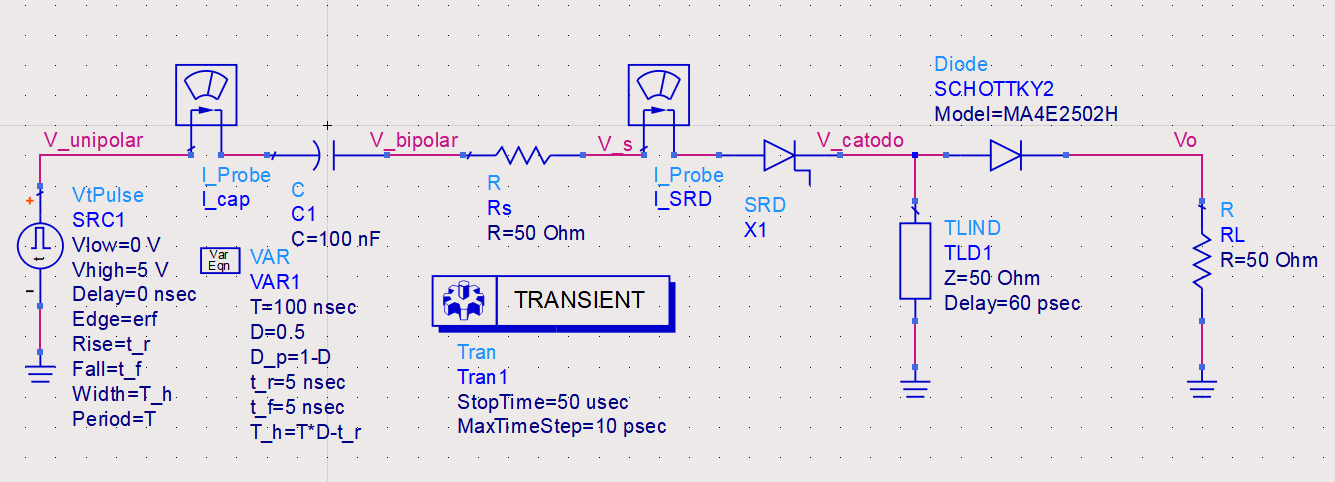
\includegraphics[width=\textwidth]{images/highpass_nonlinear_w_shunt_sch.png}
    \caption{Circuito pasa altos con carga no lineal y lineal en paralelo simulado}
    \label{fig:sch_highpass_non_linear_w_shunt_simulation}
\end{figure}

En la figura \ref{fig:highpass_non_linear_w_shunt_simulation_result} se observan
los resultados de la simulación. En este caso, a la salida se observa la
generación de pulsos. Analizando la corriente sobre el SRD, vemos que en este
caso la corriente negativa es de mayor módulo que la positiva, observándose la
transición a alta impedancia del SRD con su característica abrupta caída a $0$
de la corriente. Para la corriente en el capacitor, vemos que ahora es la suma
de la corriente en el resistor lineal y la corriente en el SRD.

\begin{figure}[tbp]
    \centering
    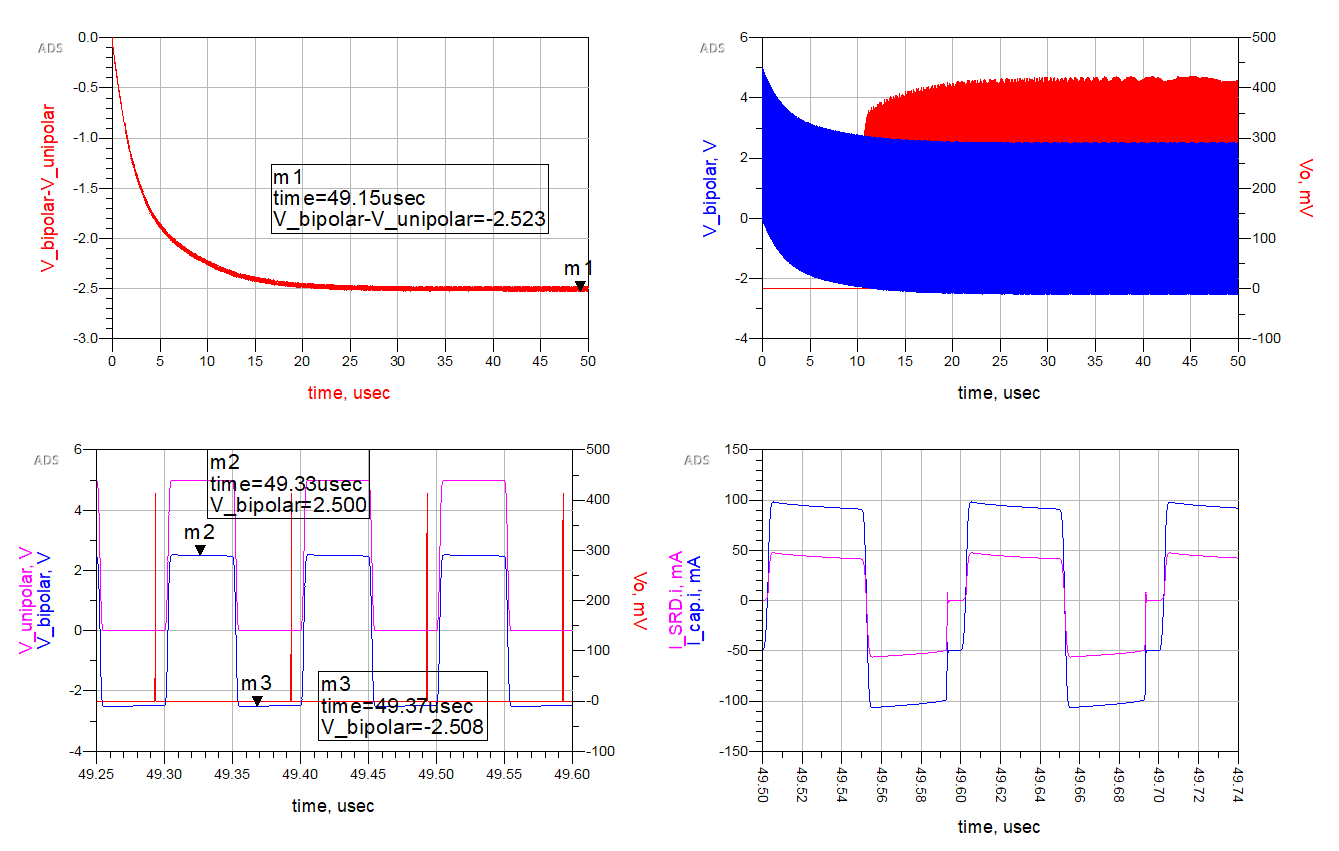
\includegraphics[width=\textwidth]{images/highpass_nonlinear_w_shunt_sim_result.png}
    \caption{Resultado de simulación de pasa altos con carga no lineal y lineal
    en paralelo.}
    \label{fig:highpass_non_linear_w_shunt_simulation_result}
\end{figure}

En cuanto a la tensión cargada en el capacitor, vemos que ahora es
\qty{-2.52}{\volt}, mayor que los \qty{-1.9}{\volt} de la simulación sin carga
lineal en paralelo. Este incremento de la tensión de carga es consistente con la
ecuación \ref{eq:vc_non_linear_load_with_shunt_final}. Evaluando la ecuación,
tenemos en este caso

\begin{equation}
    \begin{aligned}
        D &= 0.5 \\
        \gamma &= \frac{R_{sh}}{R_{sh}+R_{s}} =0.5 \\
        \alpha &= \frac{0.4}{0.5} = 0.9 \\
    \end{aligned}
\end{equation}

Donde tomamos $\alpha$ leyendo el eje $x$ de
\ref{fig:highpass_non_linear_w_shunt_simulation_result}. Para estos valores,
\ref{eq:vc_non_linear_load_with_shunt_final} predice un valor de

\begin{equation}
    \begin{aligned}
        V_C &= V_U \cdot \frac{D}{\left( 1 - \gamma \cdot D' \cdot \alpha'\right)} \\
        V_C &= \qty{5}{\volt} \cdot \frac{0.5}{\left( 1 - 0.5 \cdot (1-0.5)
        \cdot (1-0.9) \right)} \\
        V_C &= \qty{2.56}{\volt} \\
    \end{aligned}
\end{equation}

La ecuación es consistente con el resultado de la simulación. En este caso, los
valores de la señal bipolar son \qty{\pm2.5}{\volt}, habiendo logrado bajar los
niveles con respecto al resultado de la figura
\ref{fig:highpass_filter_nonlinear_load_sim_result}.

El agregado del resistor lineal en paralelo logró el efecto deseado, aumentando
la tensión en el capacitor serie, logrando una señal bipolar que logra cargar y
descargar al SRD permitiendo la generación de pulsos.

Para terminar de demostrar su funcionamiento, repetimos la simulación del
esquemático de la figura \ref{fig:highpass_nonlinear_w_shunt_sch}, ahora con un
ciclo de trabajo $D=0.8$. En la figura
\ref{fig:highpass_non_linear_w_shunt_simulation_result_80_dc} se observa el
resultado. Ahora se logra el efecto descripto anteriormente, mediante el
incremento del ciclo de trabajo $D$ decrece la tensión $V_{+}$ y aumenta
$V_{-}$, resultando en una mayor amplitud de pulso. Vemos que esta es
\qty{0.85}{\volt}, mientras que en
\ref{fig:highpass_non_linear_w_shunt_simulation_result} se obtuvieron
\qty{0.45}{\volt}.

\begin{figure}[tbp]
    \centering
    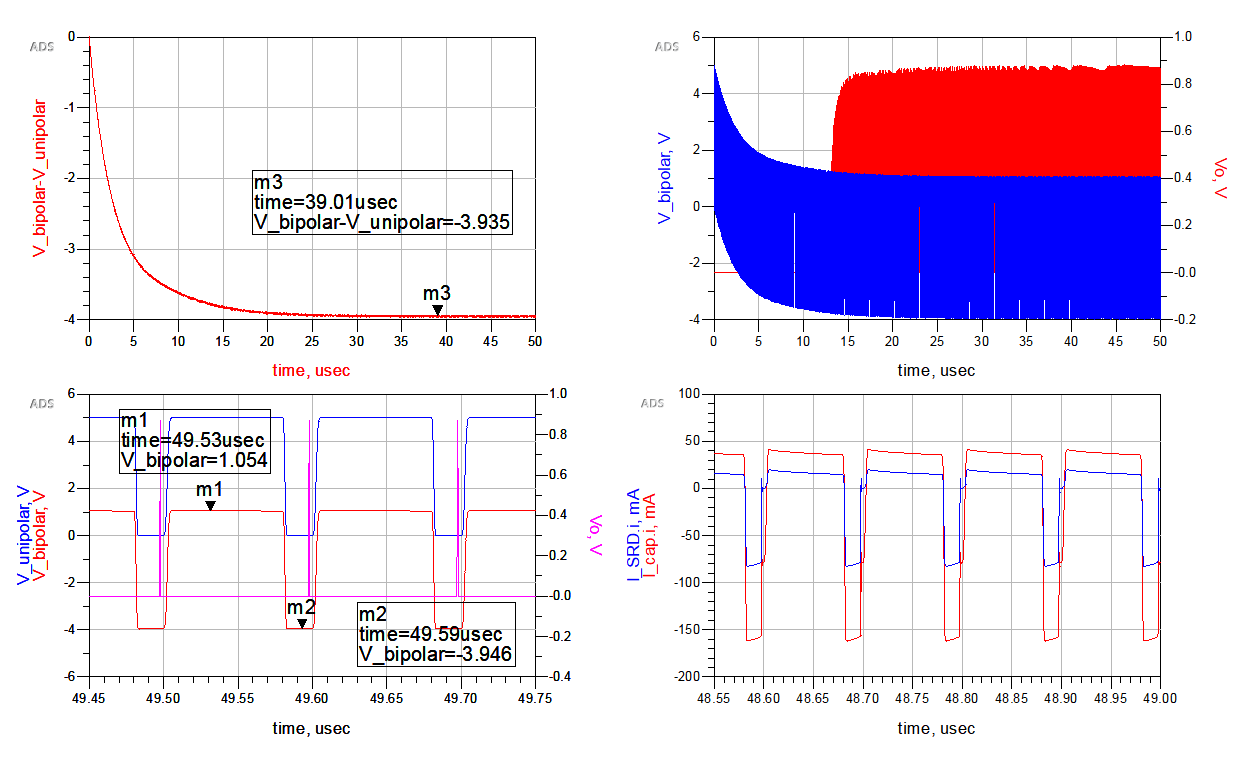
\includegraphics[width=\textwidth]{images/highpass_nonlinear_w_shunt_sim_result_80_dc.png}
    \caption{Resultado de simulación de pasa altos con carga no lineal y lineal
    en paralelo, $D=0.8$.}
    \label{fig:highpass_non_linear_w_shunt_simulation_result_80_dc}
\end{figure}

En cuanto a la tensión en el capacitor, aplicando la ecuación
\ref{eq:vc_non_linear_load_with_shunt_final}, tenemos

\begin{equation}
    \begin{aligned}
        V_C &= V_U \cdot \frac{D}{\left( 1 - \gamma \cdot D' \cdot \alpha'\right)} \\
        V_C &= \qty{5}{\volt} \cdot \frac{0.8}{\left( 1 - 0.5 \cdot (1-0.8)
        \cdot (1-0.9) \right)} \\
        V_C &= \qty{4}{\volt} \\
    \end{aligned}
\end{equation}

La ecuación se encuentra consistente con el resultado obtenido en la simulación.

\subsection{Implementación de la llave}

\subsubsection{Requisitos}

En la tabla \ref{tab:llave_requirements} se describen los requerimientos que
debe cumplir la llave

\begin{table}
\centering
\begin{tabular}{c|c}
\hline
    Variable & Requerimiento \\
\hline
    $V_{in}$                &   CMOS @ $V_{DD}=\qty{3.3}{\volt}$ ($V_{OH}$
    \qty{2.4}{\volt})     \\
    $f_{in}$                &   Typ \qty{10}{\mega\hertz} \\
    $\tau_{r}$ / $\tau_{f}$ &   Max \qty{10}{\nano\second} \\
    $V_{dd}$                &   \qty{5}{\volt} - \qty{8}{\volt} \textcolor{red}{chequear} \\
    $I_{out}$               &   Max \qty{200}{\milli\ampere} \textcolor{red}{chequear}  \\
\hline
\end{tabular}
\caption{Requerimientos de la llave para el driver.}
\label{tab:llave_requirements}
\end{table}

El requerimiento de tensión de entrada es debido al sistema objetivo de
integración del prototipo, en el que los sistemas digitales de control trabajan
con un $V_{DD}$ de \qty{3.3}{\volt}. Además, este nivel de tensión es versátil
en cuanto a que permite trabajar con otro tipo de salidas, como $TTL$
\qty{5}{\volt}.

La frecuencia de  entrada se debe a la $PRF$ objetivo de \qty{10}{\mega\hertz}.
El requerimiento de tiempo de crecimiento y caída $\tau_{r}$ / $\tau_{f}$ es
impuesto para que no sean mucho mayores a $\frac{10}{f_{in}}$. Esto garantiza
que la forma de tensión no se diferencie demasiado de la forma de onda ideal con
la que se diseñó el sistema. Es probable que formas de onda con mayores
relaciones entre tiempo de crecimiento y período funcionen para generación de
pulsos, pero para este primer prototipo se optó por una forma de onda lo más
ideal posible.

En rigor, también existe un requisito de tiempo mínimo de crecimiento/caída.
Esto se debe la presencia del stub. Como fuese explicado en
\ref{sec:generador_pulsos_stub}, el stub genera pulsos para cualquier tipo de
transición, con una amplitud de pulso proporcional a la velocidad de crecimiento
de la señal. Si los tiempos de crecimiento/caída de la llave fueran tales que el
pulso generado por el stub tenga una amplitud mayor a la tensión de encendido
del diodo Scottky, se transmitirían pulsos indeseados en la salida. Es por esto que
existe un límite inferior para el tiempo de crecimiento/caída de la llave. De
todas formas, no se impondrá  este requerimiento sobre la llave, ya que en el
circuito se dejará disponible un lugar para el soldado de un capacitor $C$
paralelo a la salida de la llave. Esto permite volver más lento el tiempo de
crecimiento en caso de que este sea demasiado rápido.

El requerimiento de $V_{dd}$ se debe al rango de tensiones de alimentación de
interés del sistema. Estas son fácilmente obtenibles en las plataformas a las
que se apunta integrar el prototipo.

\subsubsection{Llave utilizada}

En base a todos estos requerimientos, se optó por un circuito integrado
comercial \textit{gate driver}. Estos dispositivos son utilizados generalmente
para conmutar la compuerta de un transistor CMOS de potencia en base a  una
señal digital de baja capacidad de carga. Debido a la similitud entre este caso
de uso y el de este trabajo, fue fácil encontrar un dispositivo que cumpla con
los requisitos de la tabla \ref{tab:llave_requirements}.

El integrado seleccionado fue el LM5114 \cite{LM5114_datasheet}. En la figura
\ref{fig:lm5114_block_diagram} puede observarse un diagrama en bloques del
mismo, tomado de \cite{LM5114_datasheet}. El dispositivo posee dos salidas, una
para el transistor $P$ y otra para el $N$. Esto permite, mediante resistencias
externas, igualar los tiempos de crecimiento de cada transición. En nuestra
aplicación, esto no es de interés, por  lo que ambas salidas estarán
cortocircuitadas.

\begin{figure}[tbp]
    \centering
    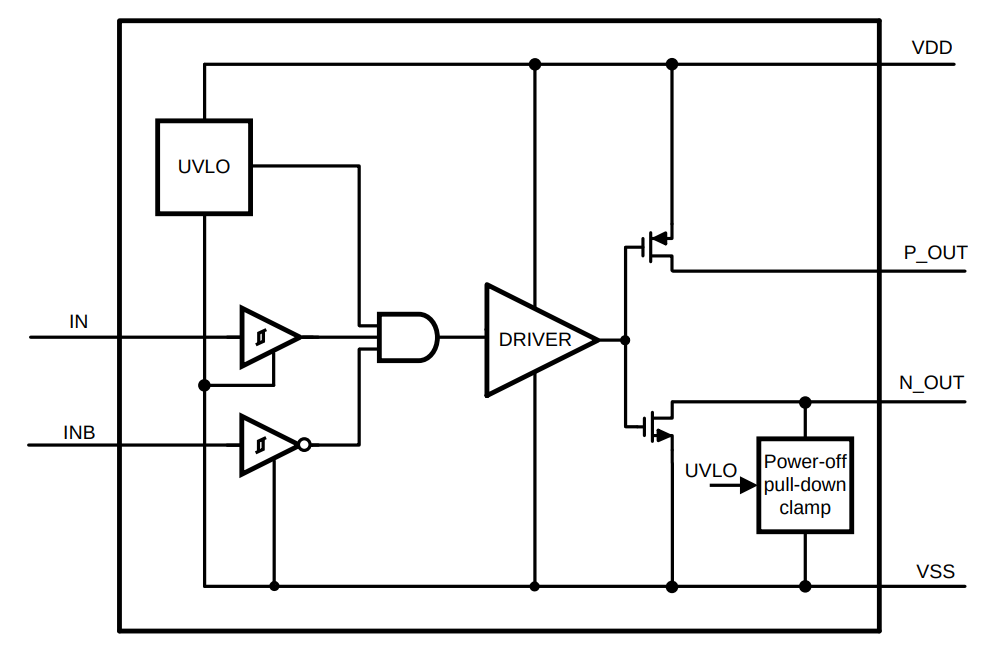
\includegraphics[width=0.4\textwidth]{images/lm5114_block_diagram.png}
    \caption{Diagrama en bloques del LM5114. Tomado de \cite{LM5114_datasheet}}
    \label{fig:lm5114_block_diagram}
\end{figure}

El integrado presenta dos versiones, $A$ y $B$, la primera teniendo niveles de
tensión de entrada CMOS y la segunda TTL.  Se optó por la versión B, ya que los
niveles de tensión CMOS dependen de la tensión de alimentación $V_{dd}$,
mientras que la TTL tiene niveles de tensión independientes de $V_{dd}$ y
compatibles con los especificados en \ref{tab:llave_requirements}. En cuanto al
encapsulado, se optó por la versión en WSON debido a su disponibilidad en
stock.

En cuanto a rango de $V_{dd}$, la hoja de datos lo especifica en \qty{4}{\volt}
- \qty{10}{\volt}, excediendo el requerimiento de \ref{tab:llave_requirements}.
No se especifica una corriente continua máxima de operación, pero se puede
obtener esta medida a partir de la especificación de máxima temperatura de
juntura $T_{jM}$ y resistencia térmica $\theta_{jA}$. Estas están especificadas en

\begin{equation}
    \begin{aligned}
        T_{jM} & = \qty{125}{\celsius} \\
        \theta_{jA} &= \qty[per-mode=fraction]{51.2}{\celsius\per\watt}
    \end{aligned}
\end{equation}

La relación entre potencia disipada $P$ en el integrado, temperatura de juntura
$T_j$, temperatura ambiente $T_A$ y resistencia térmica $\theta_{jA}$ es

\begin{equation}
    \begin{aligned}
        T_{j} = T_{A} + P \cdot \theta_{jA}
    \end{aligned}
\end{equation}

Dada la máxima temperatura de juntura $T_{jM}$, la máxima potencia $P_M$ es

\begin{equation}
    \begin{aligned}
        P_{M} = \frac{T_{jM}-T_A}{\theta_{jA}}
    \end{aligned}
\end{equation}

Aproximando el consumo de potencia en el integrado con la corriente de salida
multiplicada por la impedancia de salida, es decir, despreciando todas las otras
fuentes de disipación, tenemos

\begin{equation}
    \begin{aligned}
        P_{M} = I_{RMS_{max}}^2 \cdot R_o &= \frac{T_{jM}-T_A}{\theta_{jA}} \\
        I_{RMS_{max}} &= \sqrt{\frac{T_{jM}-T_A}{\theta_{jA}}} \cdot \frac{1}{R_o} \\
    \end{aligned}
\end{equation}

La hoja de datos especifica distintos rangos de $R_o$ para la salida $N$ y la
$P$. Utilizaremos la peor que es \qty{4.78}{\ohm}. Para $\theta_{jA}$, dado que
el valor depende no solo del integrado sino también del PCB, tomaremos un peor
caso aumentando en un \qty{50}{\percent} el especificado por el fabricante.
Entonces tenemos

\begin{equation}
    \begin{aligned}
        I_{RMS_{max}} &= \sqrt{\frac{ \qty{125}{\celsius}-
        \qty{25}{\celsius}}{\qty[per-mode=fraction]{51.2}{\celsius\per\watt}
        \cdot 1.5 }} \cdot \frac{1}{ \qty{4.78}{\ohm} } \\
        I_{RMS_{max}} &= \qty{240}{\milli\ampere}
    \end{aligned}
\end{equation}

Vemos que el requisito de la tabla \ref{tab:llave_requirements} se cumple. Cabe
destacar que esta corriente $I_M$ fue obtenida asumiendo peores casos, en caso
de requeriría una corriente superior, probablemente el integrado pueda
proveerla. Incluso en caso de exceder la corriente la temperatura máxima de
juntura, se puede colocar un disipador.

En cuanto a tiempo de caída/crecimiento $\tau_{r}$ / $\tau_{f}$, el fabricante
especifica una dependencia del mismo en función de la capacidad de carga $C_L$,
con mayores tiempos a mayor carga. Para la carga mínima especificada,
\qty{1000}{\pico\farad}, el tiempo de crecimiento es de \qty{8}{\nano\second} y
el de caída de \qty{3.2}{\nano\second}. Ambos se encuentran por debajo de los
máximos \qty{10}{\nano\second} especificados en \ref{tab:llave_requirements}.

De todas maneras, analizando la capacidad de carga que tiene el integrado, esta
es mucho menor a \qty{1000}{\pico\farad}. Como fuese explicado anteriormente, la
impedancia que presenta el pulser es igual a la resistencia $R_s$ durante el
período de conducción positivo, y $R_S/\alpha$ durante el período negativo. La
carga del gate driver está compuesta por el pulser en serie con el capacitor de
filtrado pasa altos. Este capacitor es de \qty{100}{\nano\farad}, y en las
frecuencias de trabajo de la señal cuadrada, presenta una impedancia

\begin{equation}
    \begin{aligned}
        | Z_C | &< \frac{1}{2\pi \cdot PRF \cdot C} \\
        | Z_C | &< \frac{1}{j2\pi \cdot \qty{10}{\mega\hertz} \cdot
        \qty{100}{\nano\farad}} \\
        | Z_C | &< \qty{15}{\milli\ohm}
    \end{aligned}
\end{equation}

La impedancia del capacitor es menor en todo el rango ya que el contenido
espectral de la señal cuadrada se encuentra por arriba de la frecuencia
fundamental $PRF$. Entonces, la impedancia de carga del gate driver es $Z_L
\approx \qty{50}{\ohm} + j \cdot \qty{15}{\milli\ohm} \approx \qty{50}{\ohm}$,
es decir una carga resistiva pura, debido a lo despreciable de la impedancia del
capacitor serie con la resistencia de limitación de corriente $R_s$. En este
análisis no se tuvieron en cuenta las capacidades a tierra parásitas tanto de
los encapsulados como del PCB, por lo que serán estas las que determinen la
capacidad de carga real.

Se encuentra especificada una asimetría importante entre $\tau_r$ y $\tau_f$,
siendo el último aproximadamente un \qty{25}{\percent} del primero. Esta
asimetría es un sentido beneficioso para el circuito, ya que el tiempo de
transición crítico es el de caída. Este tiempo tiene que ser lo suficientemente
rápido para que cuando el SRD transiciones al estado de alta impedancia, la forma
de onda de entrada ya haya llegado a su mínimo valor. Caso contrario, el pulso
tendrá menor amplitud. Esto es claro de la ecuación \ref{eq:A_p}, donde se
establece que la amplitud del pulso es directamente proporcional a la tensión en
el ánodo del SRD.

El dispositivo no presenta una especificación de frecuencia de trabajo, pero
contiene especificaciones de tiempo de propagación y tiempos de
caída/crecimiento, que imponen una restricción sobre la máxima frecuencia de
operación. En la figura \ref{fig:lm5114_timing_definitions} se observan las
definiciones de tiempo de propagación y caída/crecimiento. De la definición, el
tiempo desde que la señal de entrada llega a un \qty{50}{\percent} hasta que la
salida conmuta es aproximadamente $t_{D-on}+t_{r}$ para el caso de una
transición $0\to1$, y para la transición $1\to0$ será $t_{D-off}+t_{f}$.

\begin{figure}[tbp]
    \centering
    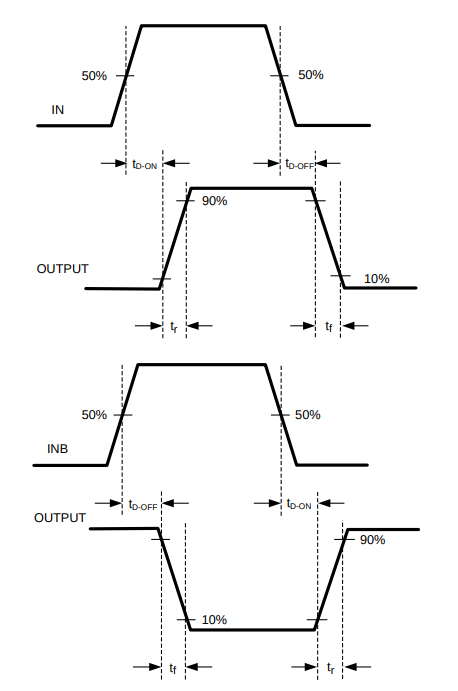
\includegraphics[width=0.4\textwidth]{images/lm5114_timing_definitions.png}
    \caption{Definición de tiempos de transición y propagación, tomado de
    \cite{LM5114_datasheet}}
    \label{fig:lm5114_timing_definitions}
\end{figure}

Referenciando estos al inicio de la transición de la señal de entrada, tenemos
que son $t_{ri}+t_{D-on}+t_{ro}$ y $t_{fi}+t_{D-off}+t_{fo}$, donde definimos a
$t_{ri}$ y $t_{fi}$ y $t_{ro}$ y $t_{fo}$ como los tiempos de transición
$\qty{10}{\percent}-\qty{90}{\percent}$ de las señales de entrada y salida
respectivamente. Estas expresiones son cotas superiores, ya que los tiempos de
crecimiento son del \qty{10}{\percent} al \qty{90}{\percent}, mientras que el
tiempo anterior estaba reverenciado desde el \qty{50}{\percent} de la señal de
entrada.

Entonces, vemos que el período mínimo será $T_{min} = t_{ri} + t_{D-on} + t_{ro}
+ t_{fi} + t_{D-off} + t_{fo}$. De la hoja de datos, tenemos los siguientes
peores (máximos) tiempos especificados para operación a $T_j=\qty{25}{\celsius}$

\begin{itemize}
    \item $t_{D-on} = \qty{27}{\nano\second}$
    \item $t_{r} @ \qty{1000}{\pico\farad} = \qty{12}{\nano\second}$
    \item $t_{D-off} = \qty{27}{\nano\second}$
    \item $t_{f} @ \qty{1000}{\pico\farad} = \qty{3}{\nano\second}$
\end{itemize}

Asumiendo para un peor caso, tiempos de transición de entrada de
\qty{10}{\nano\second},  tenemos un período mínimo de

\begin{equation}
    \begin{aligned}
        T_{min} &= t_{ri} + t_{D-on} + t_{ro} + t_{fi} + t_{D-off} + t_{fo} \\
        T_{min} &= \qty{10}{\nano\second} + \qty{27}{\nano\second} +
        \qty{12}{\nano\second} + \qty{10}{\nano\second} + \qty{27}{\nano\second}
        + \qty{3}{\nano\second} \\
        T_{min} &= \qty{89}{\nano\second} \\
    \end{aligned}
\end{equation}

El período mínimo se encuentra por debajo del período de \qty{100}{\nano\second}
correspondiente a los \qty{10}{\mega\hertz} especificados en
la tabla \ref{tab:llave_requirements}, por lo que se cumple el requerimiento de $f_{in}$.

\subsubsection{Simulación}

El fabricante provee un modelo de SPICE del gate driver \cite{LM5114-PSpice}.
Con este se realizó una simulación para confirmar el correcto funcionamiento. En
la figura \ref{fig:lm5114_sim_sch} puede observarse el esquemático simulado. El
mismo consiste en el pulser, el capacitor de filtrado pasa altos, y el LM5114
junto a una fuente cuadrada unipolar de \qty{3.3}{\volt}. Esta simula la señal
de control del sistema embebido de bajo costo.

La simulación se realiza bajo dos condiciones de ciclo de trabajo para la señal
de entrada: \qty{50}{\percent}, con el resultado en la figura
\ref{fig:lm5114_sim_result_50_D} y \qty{70}{\percent}, resultado en la figura
\ref{fig:lm5114_sim_result_70_D}. En ambos casos se observa la transición del
SRD al estado de alta impedancia y la consecuente generación de pulsos. Se
observa que en este caso la señal cuadrada unipolar no tiene la amplitud
completa de la fuente de alimentación, \qty{5}{\volt}, sino aproximadamente
\qty{4.5}{\volt}, debido a las perdidas en el LM5114. Se observa que el efecto
de aumentar el ciclo de trabajo de \qty{50}{\percent} a \qty{70}{\percent} logra
un aumento en la amplitud del pulso de casi un \qty{100}{\percent} como en la
sección anterior.

\begin{figure}[tbp]
    \centering
    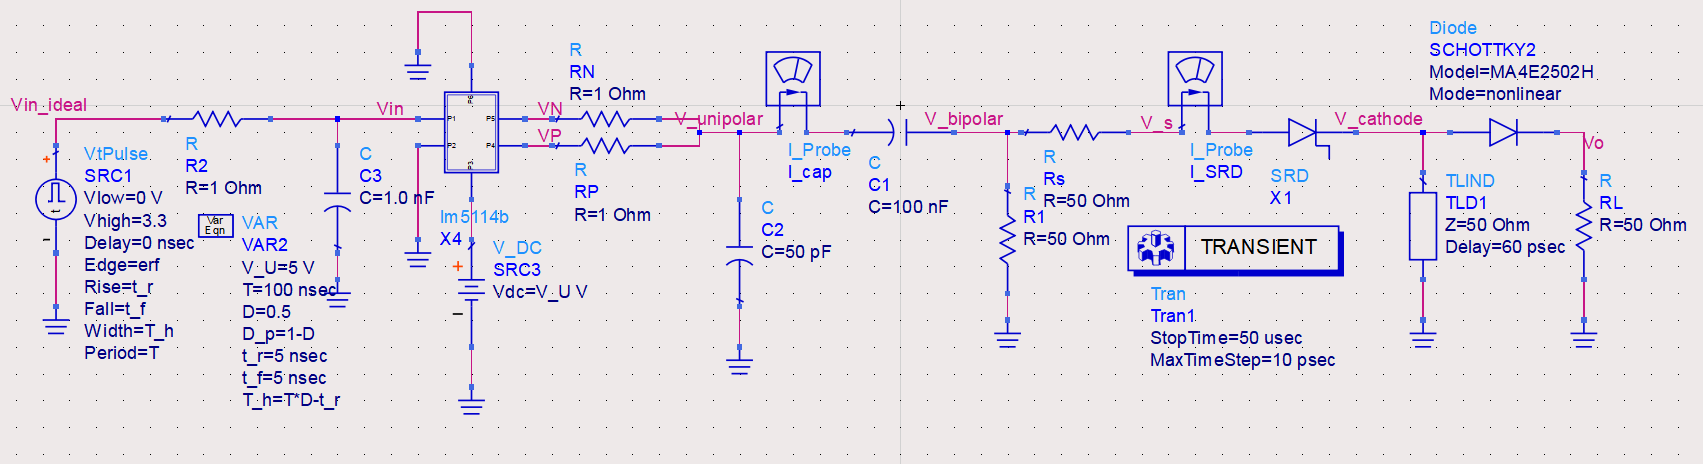
\includegraphics[width=\textwidth]{images/lm5114_sim_sch.png}
    \caption{Esquemático de simulación con modelo de LM5114.}
    \label{fig:lm5114_sim_sch}
\end{figure}

\begin{figure}[tbp]
    \centering
    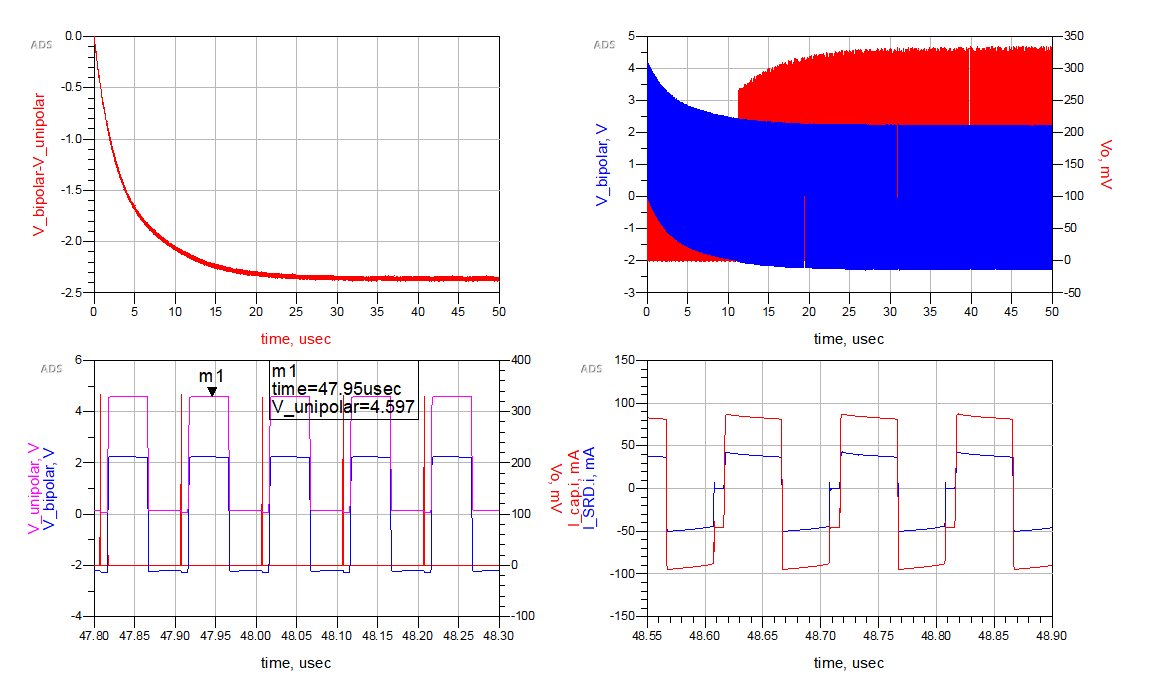
\includegraphics[width=\textwidth]{images/lm5114_sim_result_50_D.png}
    \caption{Resultado de simulación con modelo de LM5114, $D=0.5$.}
    \label{fig:lm5114_sim_result_50_D}
\end{figure}

\begin{figure}[tbp]
    \centering
    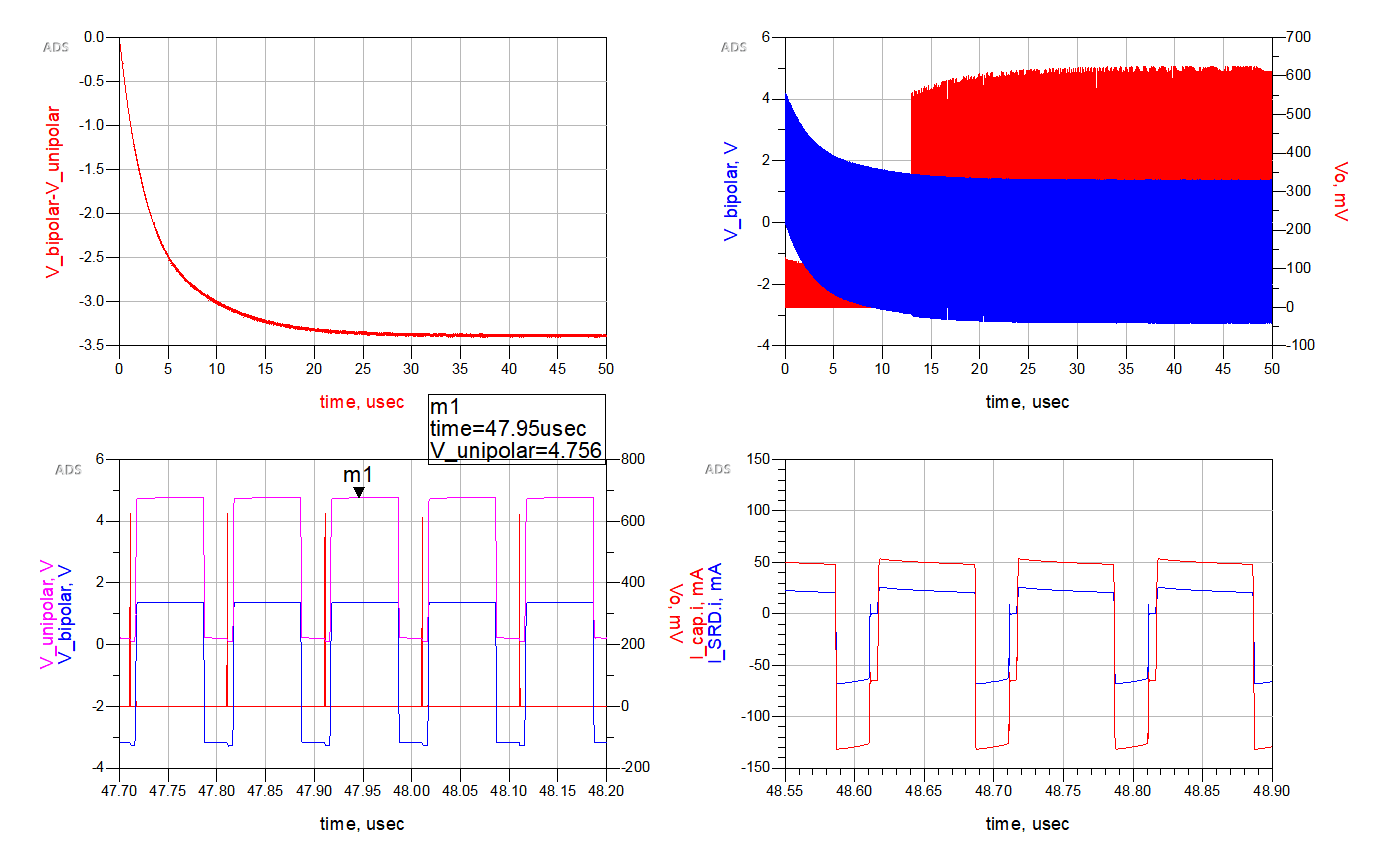
\includegraphics[width=\textwidth]{images/lm5114_sim_result_70_D.png}
    \caption{Resultado de simulación con modelo de LM5114, $D=0.7$.}
    \label{fig:lm5114_sim_result_70_D}
\end{figure}

\section{Implementación en PCB}

Se implementó en PCB el circuito diseñado. Se diseñaron dos placas distintas:
una para el driver, y otra para el pulser. Se tomó esta decisión para darle más
versatilidad al trabajo. De esta manera, el pulser puede utilizarse con otro
eventual driver, el driver puede ser evaluado por separado antes de una medición
final, y en caso de falla de diseño en alguno de los dos circuitos, la falla se
mantiene contenida al modulo defectuoso y no a la totalidad del sistema.

Se fabricaron las placas con el fabricante OSHPark. Se utilizó el servicio de 4
capas y material FR408HR de Isola \cite{fr408_datasheet}. El material, a
diferencia del FR4 más económico, presenta buena estabilidad en frecuencia para
su constante dieléctrica y bajas perdidas, por lo que es apropiado para
trabajar en el ancho de banda necesario. La constante dieléctrica presenta una
variación menor al \qty{2}{\percent} en el rango \qty{100}{\mega\hertz} a
\qty{10}{\giga\hertz}, y una tangente de pérdidas con mayor variación pero menor
a \num{0.01} hasta \qty{10}{\giga\hertz}.

En la tabla \ref{tab:oshpark_4_layer_stackup} se muestra el apilamiento de las
capas del proceso de fabricación, con sus dimensiones y materiales. El proceso
consta de 4 capas conductoras, todas compuestas por cobre. Entre ambos pares de
conductores se encuentra el \textit{prepeg} de constante dieléctrica estable en
frecuencia. Entre los dos pares se encuentra el núcleo FR4. Por sobre las capas de
cobre superior e inferior se encuentran capas de serigrafía y máscaras de
soldadura, que a los efectos de cálculos de impedancia tienen un rol
despreciable.

\textcolor{red}{comentar q usamos la de 4 capas porque tenía un H más chico? xq
era esto?}

\begin{table}[htbp]
\centering
\begin{threeparttable}[b]
    \begin{tabular}{c|c|c|c}
        Capa & C/D \tnote{a} & Grosor [mil]  & $\epsilon_r$ \tnote{b} \\
        \hline
        Serigrafía & D & 1 $\pm$0.2 & \\
        Máscara de soldadura & D & 1 $\pm$0.2 & \\
        Cobre 1 oz & C & 1.7 \\
        \textit{Prepreg} FR408HR 2113  & D & 7.96 $\pm$0.796 &
        3.61@\qty{1}{\giga\hertz} \\
        Cobre 0.5 oz & C & 0.68 & \\
        Núcleo FR408HR & D & 39 $\pm$3.9 & \\
        Cobre 0.5 & C & 0.68 \\
        \textit{Prepreg} FR408HR 2113 & D & 7.96 $\pm$0.796 &
        3.61@\qty{1}{\giga\hertz}\\
        Cobre 1 oz & C & 1.7 & \\
        Máscara de soldadura & D & 1 $\pm$0.2 & \\
        Serigrafía & D & 1 $\pm$0.2 & \\
    \end{tabular}
    \begin{tablenotes}
        \item [a] Conductor/Dieléctrico.
        \item [a] Permisividad relativa.
    \end{tablenotes}
\end{threeparttable}
\caption{Apilamiento de capas del proceso de fabricación de OSH Park}
\label{tab:oshpark_4_layer_stackup}
\end{table}

\subsection{Selección de componentes pasivos}

Hablar de que se apuntó a usar componentes lo más pequeños posibles para
eliminar las contribuciones de las impedancias parásitas

\subsection{Layout del pulser}

Para el pulser, se utilizó la capa superior de cobre como plano de señal y la
capa de cobre inferior a esta como tierra. De esta manera, se forma un linea de
transmisión microtira \cite{pozar2011}, siendo el material dieléctrico el
\textit{prepeg} de permisividad relativa estable en frecuencia y una altura de
$H = \qty{7.96}{\mil} = \qty{0.0202}{\milli\meter}$.

Dado el $H$ de la línea de transmisión, se calculó el $w$ necesario para obtener
una impedancia característica de \qty{50}{\ohm}. Para esto, se utilizo el
programa \textit{LineCalc} disponible dentro de \textit{ADS}. Este programa
permite cargar una configuración de línea de transmisión, y en base al alto del
dieléctrico $H$ y una impedancia característica deseada $Z_o$, obtener el ancho
$w$ necesario. En la figura \ref{fig:tline_width_calculation} se observan los
parámetros configurados. Esto resultó en un ancho de pista de
\qty{0.4}{\milli\meter}.

\begin{figure}[tbp]
    \centering
    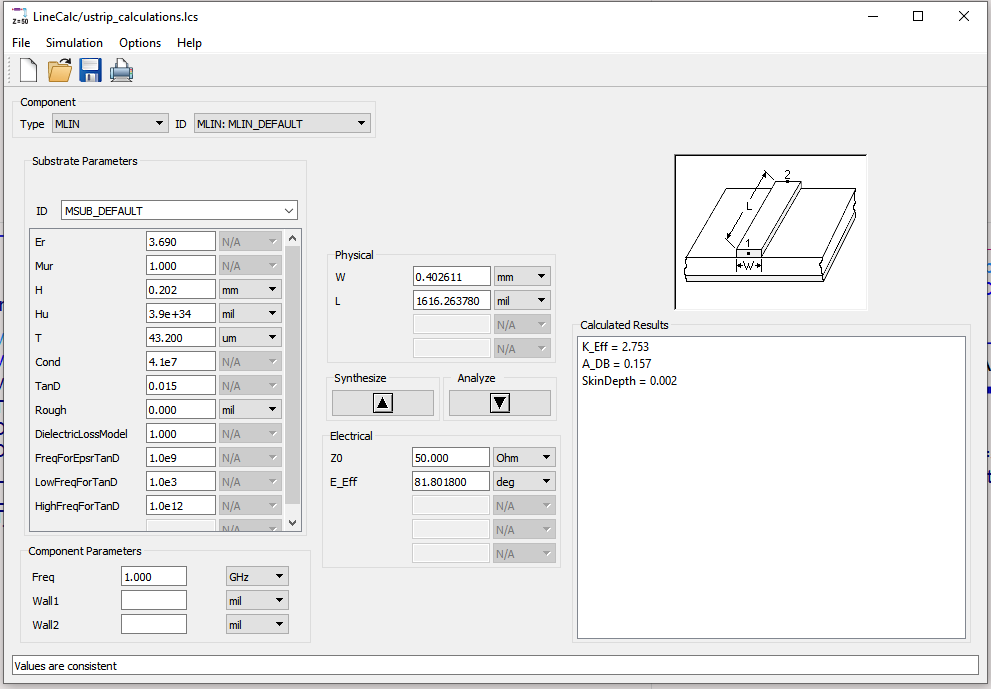
\includegraphics[width=0.6\textwidth]{images/tline_width_calculation.png}
    \caption{Calculo de línea de transmisión para obtener \qty{50}{\ohm}.}
    \label{fig:tline_width_calculation}
\end{figure}

\subsubsection{Diseño del \textit{stub}}

Con la línea de transmisión a utilizar en el pulser determinada como una
microtira de los parámetros dados por el proceso de fabricación de la tabla
\ref{tab:oshpark_4_layer_stackup}, se obtuvo su $\kappa_{eff}$ con el programa
\textit{LineCalc}. En la figura \ref{fig:tline_width_calculation} se observa que
este es de \num{2.753}.

Reemplazando estos datos en la ecuación \ref{eq:stub_length_vs_delay} podemos
obtener el largo necesario para obtener un retardo de \qty{60}{\pico\second}.

\begin{equation}
    \begin{aligned}
        L &= \frac{T_p}{2} \cdot \frac{c_0}{\sqrt{\kappa_{eff}}} \\
        L &= \frac{\qty{120}{\pico\second}}{2} \cdot \frac{
            \qty{3e8}{\meter\per\second}}{\sqrt{2.753}} \\
        L &= \qty{10.85}{\milli\meter}
    \end{aligned}
\end{equation}

\subsubsection{Layout}

Una vez diseñada la línea de transmisión y simulada en \textit{ADS}, se exportó
el layout obtenido en formato \textit{Gerber}. Este fue importado en el software
de código abierto \textit{KiCad}, donde se realizaron cuestiones finales. En la
figura \ref{fig:pulser_layout} puede observarse el resultado.

\begin{figure}[tbp]
    \centering
    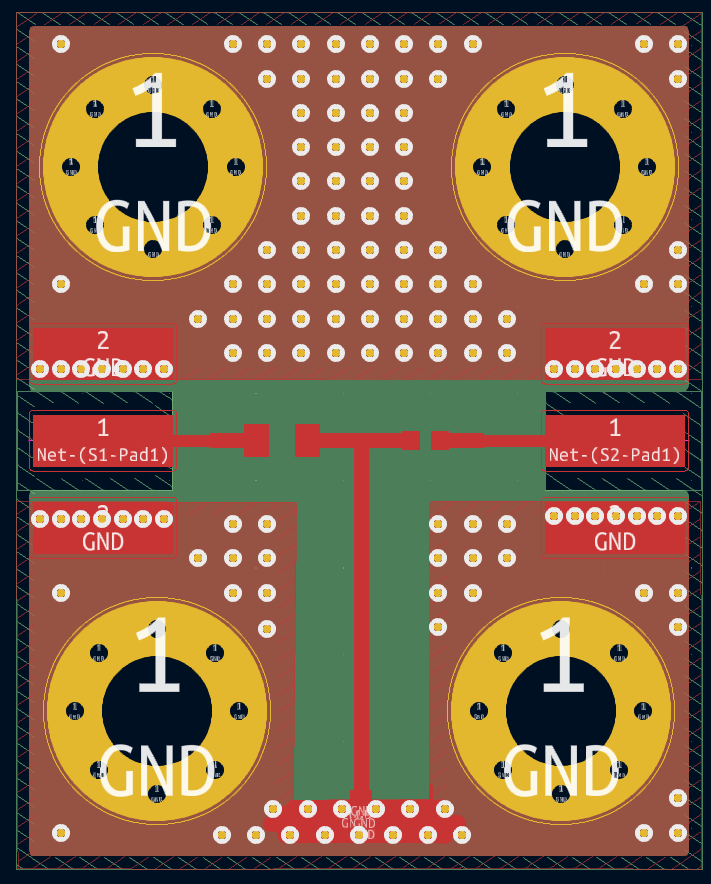
\includegraphics[width=0.6\textwidth]{images/pulser_layout.png}
    \caption{Captura del PCB diseñado en \textit{KiCad}.}
    \label{fig:pulser_layout}
\end{figure}

Se agregaron conectores \textit{SMA} para la entrada y salida
\textcolor{red}{explicar por qué SMA?}. Para mejorar el ancho de banda de la
transición, se realizó un tappering en el plano de tierra
\textcolor{red}{explicar mejor esto, buscar el mail donde Andrés recomendó
hacerlo}.

Se agregaron agujeros de montaje en los 4 extremos de la placa. También se dejó
un espacio al costado, para después poner un chasis alrededor de la placa.

En todo el plano se agregaron vías, con una separación de \textcolor{red}{XXX
mm}. Estas mejoran la puesta a tierra de todo el plano, reduciendo la impedancia
del mismo.

\textcolor{red}{se hizo un tappering desde el pad hasta el conector SMA? o fue
por error?}

En las capas inferior e intermedia 2 se usaron de plano de tierra,

Se utilizaron componentes pequeños. Se pusieron muchas vias. Se hizo un
tappering con los conectores SMA?

\subsection{Layout del driver}

Mostrar el layout del driver, explicar por qué se hizo así.

Explicar lo del integrado para filtrar el ruido. Explicar que había un jumper
para alimentación externa. Explicar que se usó PMOD para conectar a la FPGA.

Mostrar que se dejó un espacio para el capacitor paralelo en el LM114 para
reducir el tiempo de crecimient. Al final no fue necesario.

Explicar que se armó una plaquita para filtrar ruido de manera externa?

\subsection{Simulación con parásitos extraídos}

\section{Fabricación}

Explicar algo sobre la fabricación? Complicaciones con los componentes chicos?
O agregar al capitulo 4?
